\documentclass[12pt]{article}

\usepackage{graphicx,psfrag,epsf}
%\usepackage[margin=0.7in,footskip=0.2in]{geometry}%big footskip brings number down, small footskip brings number up
\usepackage{amsmath}
\usepackage{amssymb}
\usepackage[T1]{fontenc}
\usepackage{listings}
\usepackage{bm}
\usepackage{hyperref}
\usepackage{setspace}
\usepackage[usenames]{color}
\usepackage[utf8]{inputenc}
\usepackage{wrapfig}
\usepackage{relsize}
\usepackage{psfrag}
\usepackage{dsfont}
\usepackage{bbding}
\usepackage{caption}
\usepackage{natbib}
\usepackage{url}
\usepackage{fancyvrb}

\hypersetup{colorlinks   = true, %Colors links instead of ugly boxes
            urlcolor     = black, %Color for external hyperlinks
            citecolor    = blue,
            linkcolor    = black
}

\addtolength{\oddsidemargin}{-.5in}%
\addtolength{\evensidemargin}{-.5in}%
\addtolength{\textwidth}{1in}%
\addtolength{\textheight}{1.3in}%
\addtolength{\topmargin}{-.8in}%

\pdfminorversion=4

%1: Blind; 0: Sighted
\newcommand{\blind}{0}

\renewcommand*\contentsname{Table of Contents}

\newcommand{\E}[1]{
        \mathbb{E}\left[~#1~\right]
}

\def \oner {
        \mathlarger{\mathds{1}}
}

\newcommand{\argmin}{\operatornamewithlimits{argmin}}
\newcommand{\argmax}{\operatornamewithlimits{argmax}}
\newcommand*{\approxdist}{\mathrel{\vcenter{\offinterlineskip
\vskip-.25ex\hbox{\hskip.55ex$\cdot$}\vskip-.25ex\hbox{$\sim$}
\vskip-.5ex\hbox{\hskip.55ex$\cdot$}}}}
%\def\checkmark{\tikz\fill[scale=0.4](0,.35) -- (.25,0) -- (1,.7) -- (.25,.15) -- cycle;} 
%\DeclareMathOperator*{\argmax}{arg\,max}


\def \Eix {
        \mathbb{E}\left[~\text{I}(\bm{x})~\right]
}

\def \EIx {
        \mathbb{E}\left[~\text{I}(\underline{\bm{x}})~\right]
}

\def \Ix {
        \text{I}(\underline{\bm{x}})
}

\def \ix {
        \text{I}(\bm{x})
}

\def \roseVar {
	0.35 %0.06%
}

\def \roseLamb {
        0.5     
}

\def \rastVar {
        1.71 %0.88 %
}

\def \rastLamb {
        0.4
}

\def \lockVar {
        2.86 %1.97 %
}

\def \lockLamb {
        0.4
}

\begin{document}
\def\spacingset#1{\renewcommand{\baselinestretch}%
{#1}\small\normalsize} \spacingset{1}

%
%
\if0\blind
{
\title{{\LARGE\bf Determining Convergence in Gaussian Process Surrogate Model Optimization}}
\author{Nicholas R. Grunloh\\ %\thanks{The authors gratefully acknowledge}\hspace{.2cm}\\
    Department of Applied Mathematics and Statistics,\\ University of California, Santa Cruz\\
    and \\
    Herbert K. H. Lee \\
    Department of Applied Mathematics and Statistics,\\ University of California, Santa Cruz
}
%
%\title{\bf Title}
%  \author{Author 1\thanks{
%    The authors gratefully acknowledge}\hspace{.2cm}\\
%    Department of YYY, University of XXX\\
%    and \\
%    Author 2 \\
%    Department of ZZZ, University of WWW}
  \maketitle
} \fi

\if1\blind
{
  \bigskip
  \bigskip
  \bigskip
  \begin{center}
    {\LARGE\bf Determining Convergence in Gaussian Process Surrogate Model Optimization}
  \end{center}
  \medskip
} \fi

%\bigskip
%\begin{abstract}
%The text of your abstract.  100 or fewer words.
%\end{abstract}
%
%\noindent%
%{\it Keywords:}  3 to 6 keywords, (don't reuse words appearing in title)
%\vfill
%\hfill {\tiny technometrics tex template (do not remove)}
%%
%%

%% 
%%
%\title{Assessing Convergence in Gaussian Process Surrogate Model Optimization}
%\author{Nicholas R. Grunloh and Herbert K. H. Lee}
%\date{}
%\maketitle
%%
%%

%
% \newgeometry{ margin=1in, top=0.70in, footskip=0.4in }
\bigskip
\begin{abstract}
\noindent
%due to the subjective nature of convergence 
Identifying convergence in numerical optimization is an ever-present, difficult, and often subjective task. 
%, sequential design, secondary
The statistical framework of Gaussian process surrogate model optimization provides useful measures for tracking optimization progress; however, the identification of convergence via these criteria has often provided only limited success and often requires a more subjective analysis. % it these measures still subjective. % that can be used to identify convergence. 
%to track the expected improvement criterion to make
Here we develop a novel approach using ideas originally introduced in the field of statistical process control to define a robust convergence criterion based upon the improvement function. 
% to remove this subjectivity from the identification of convergence.
The Exponentially Weighted Moving Average (EWMA) chart provides an ideal starting point for adaptation to track convergence via the EWMA convergence chart introduced here.
\end{abstract}

\noindent
{\it Keywords:} Derivative-free Optimization, Computer Simulation, Emulator, Expected Improvement. EWMA
\vfill

\clearpage
\spacingset{1.45}

%
%
\section{Introduction}
%
%

%% ______ a wide range of objective function applications.
%%notable {\color{red}In the absence of derivative information, numerical optimization} is a 
%%Derivative-free optimization's independence; optimization routine
%%In the world of derivative-free optimization; In the absence of derivative information derivative-free
%Releasing numerical optimization from its dependence on derivative information, has made black-box optimization a powerful and flexible tool for solving a wide range of engineering problems.
%%
%Of primary interest here, is the application of derivative-free optimization on computationally expensive black-box objective functions, such as computer simulations.
%%{\color{red}, in the real world}
%Often computer simulations can function as fast, cost-effective, development test beds for processes that are otherwise too expensive, or dangerous, to test physically. 
%% complex case study
%For example, the Lockwood pump-and-treat simulator, discussed in more detail in section {\color{red}XX}, computationally simulates the flow of contaminated groundwater alongside the Yellowstone River as numerical solutions to coupled systems {\color{red}cite}.
%%, as efficiently as possible control
%The focus of the Lockwood simulation is to optimize the management of this contaminated groundwater flow, so as to avoid contamination of the river.
%%control schemes
%However, the space of possible management schemes is large, and it is hard to identify when derivative-free optimization has converged to an optimal solution.
%%Due to the computational expense of such simulators, it is often desirable to optimize while evaluating the simulation as seldomly as possible, without sacrificing the quality of the solution.
%Due to the computational expense of such simulators, it is desirable to do effective optimization with as few simulation evaluations as possible.
%%This is achieved; The idea is to achieve this end
%This is achieved by efficiently exploring the solution space and limiting the number of function evaluations by robustly recognizing convergence.

%
%

%is an important problem with
Black-box derivative-free optimization has a
wide variety of applications, especially in the realm of computer
simulations \citep{KoldLewiTorc2003,gramacy2014}.  
%
When dealing with computationally expensive computer
models, a key question is that of convergence of the optimization.
%
Because each function evaluation is expensive, one wants to terminate
the optimization as early as possible.  
%
However for complex simulators, the response surface may be ill-behaved and optimization
routines can easily become trapped in a local mode, so one needs to
run the optimization sufficiently long to achieve a robust solution.
%
So far there have been no reliable solutions for assessing convergence of surrogate model optimization.
In this paper, we provide an automated method for determining convergence of 
Gaussian process surrogate model optimization by bringing in elements
of Statistical Process Control.

%
%

%
Our motivating example is a hydrology application, the Lockwood
pump-and-treat problem \citep{lockCite}, discussed in more detail in Section~\ref{sec:lockwood}, wherein contamination in the groundwater near the
Yellowstone River is remediated via a set of treatment wells.  
%
The goal is to minimize the cost of running the wells while ensuring that
no contamination enters the river.  
%
The contamination constraint results in a complicated boundary that is unknown in advance and
requires evaluation of the simulator. %, and thus 
%
Finding the global constrained minimum is a difficult problem where it is easy for
optimization routines to temporarily get stuck in a local
minimum. (Gaussian process surrogate model optimization should eventually escape local minima if run long enough.)  
%
Without knowing the answer in advance, how do we know when
to terminate the optimization routine?


%
%

%related to; is often employed for optimization of computer simulation experiments.
%, a relatively quick, statistical model of the objective function output; this model serves as surrogate of the objective function itself and .
The context of this paper is Gaussian process (GP) surrogate model
optimization, a statistical modeling approach to derivative-free
numerical optimization that constructs a fast approximation to
the expensive computer simulation output surface using a statistical surrogate model \citep{santnerBook}.
%
%The surrogate model is relatively fast to work with, as compared with a large computer simulation, and 
Analysis of the surrogate model allows for efficient exploration the objective solution space.  
%
Typically a Gaussian process surrogate model is chosen for its
robustness, relative ease of computation, and its predictive framework.
%   landscape of the simulation parameters assessing future points of exploration on
Arising naturally from the GP predictive distribution \citep{gBook}, the maximum Expectation of the Improvement distribution (EI) has shown to be a valuable criterion for guiding the exploration of the objective function and shows promise for use as a convergence criterion \citep{jonesEIOpt, taddyOpt}. %furthermore the EI shows promise for use as a convergence criterion {\color{red}cite}.
%The maximum Expected Improvement (EI) criterion has shown to be a valuable criterion, arising naturally from the GP predictive distribution {\color{red}cite}.
%
% The EI criterion can be used to assess future points of exploration on the objective function, as well as for monitoring the overall convergence of the optimization routine at large {\color{red}cite}.
% As such, the evaluation of the simulator is often the rate-limiting step for numerical optimization.


%
%

%\clearpage
%however; as a means of assessing convergence GP surrogate
%{\color{red}Literature cite} recommends considering the EI as a convergence criterion for surrogate model optimization; as of yet, little work has been done to describe what convergence of these algorithms actually looks like in the context of the EI criterion.
\cite{taddyOpt} considers the use of the improvement distribution for identifying global convergence; stating its value for use in applied optimization.
%, but it has not yet been established if there is some threshold EI value that is sufficient
The basic idea behind the use of improvement in identifying convergence is that convergence should occur when the surrogate model produces low expectations for discovering a new optimum; that is to say, globally small EI values should be associated with convergence of the algorithm.
%claim that there exists 
Thus a simplistic stopping rule might first define some lower EI threshold, then claim convergence upon the first instance of an EI value falling below this threshold, as seen in \cite{windExample}.    
%in many different; of many other numerical optimization routines; that have been designed specifically to exhibit such behavior upon convergence  
This use of EI as a convergence criterion is analogous to other standard convergence identification methods in numerical optimization (e.g., the vanishing step sizes of a Newton-Raphson algorithm).
%
However, applying this same threshold strategy to the convergence of surrogate model optimization has not yet been adequately justified.
%, derived from the predictive distribution of the underling GP model; behavior
In fact, this use of EI ignores the nature of the EI criterion as a random variable, and oversimplifies the stochastic nature of convergence in this setting.
%
Thus it is no surprise that this treatment of the EI criterion can result in an inconsistent stopping rule as demonstrated in \mbox{Figure (\ref{introFig}).}  

%\clearpage
%
%
\begin{figure}[htb]
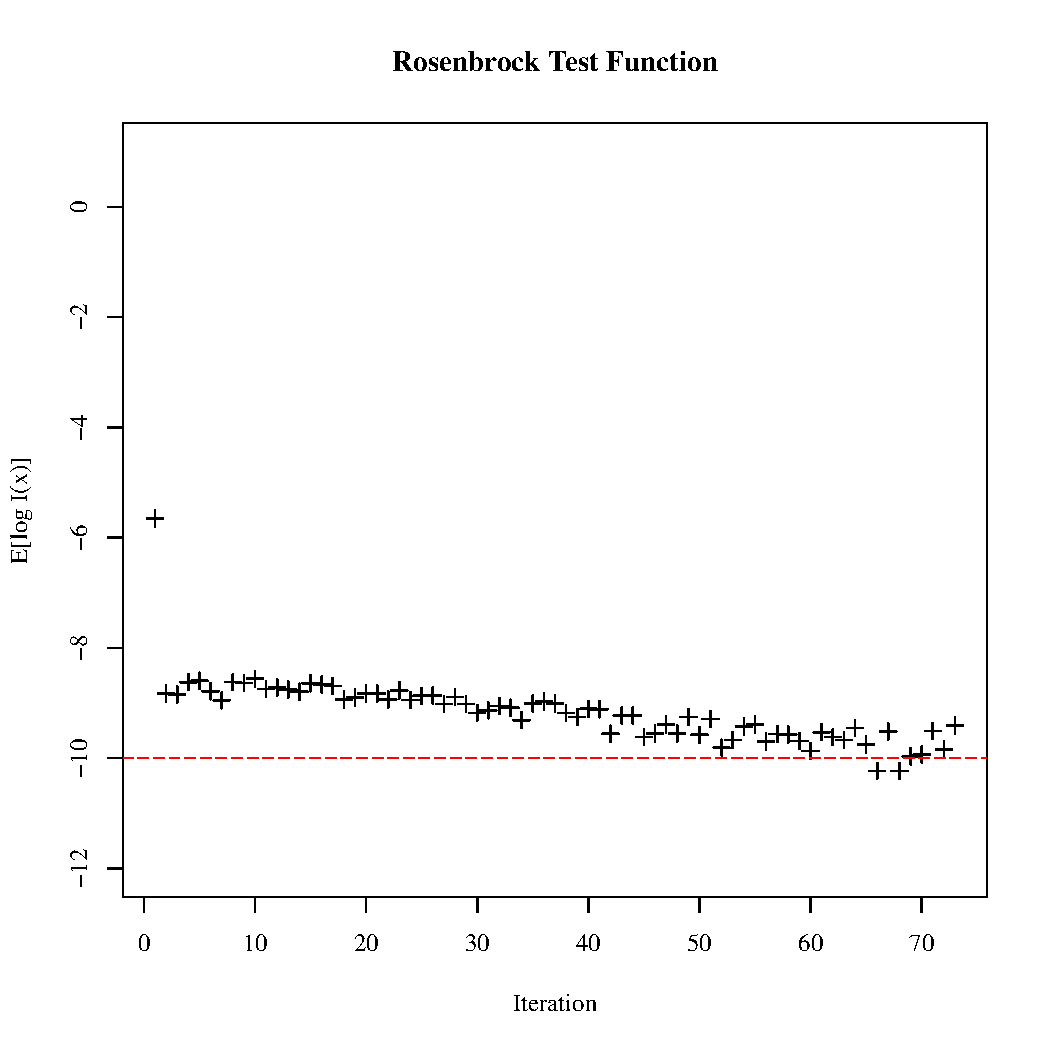
\includegraphics[width=0.32\textwidth]{./figures/introChartRoseEasyEasyAxis.pdf}
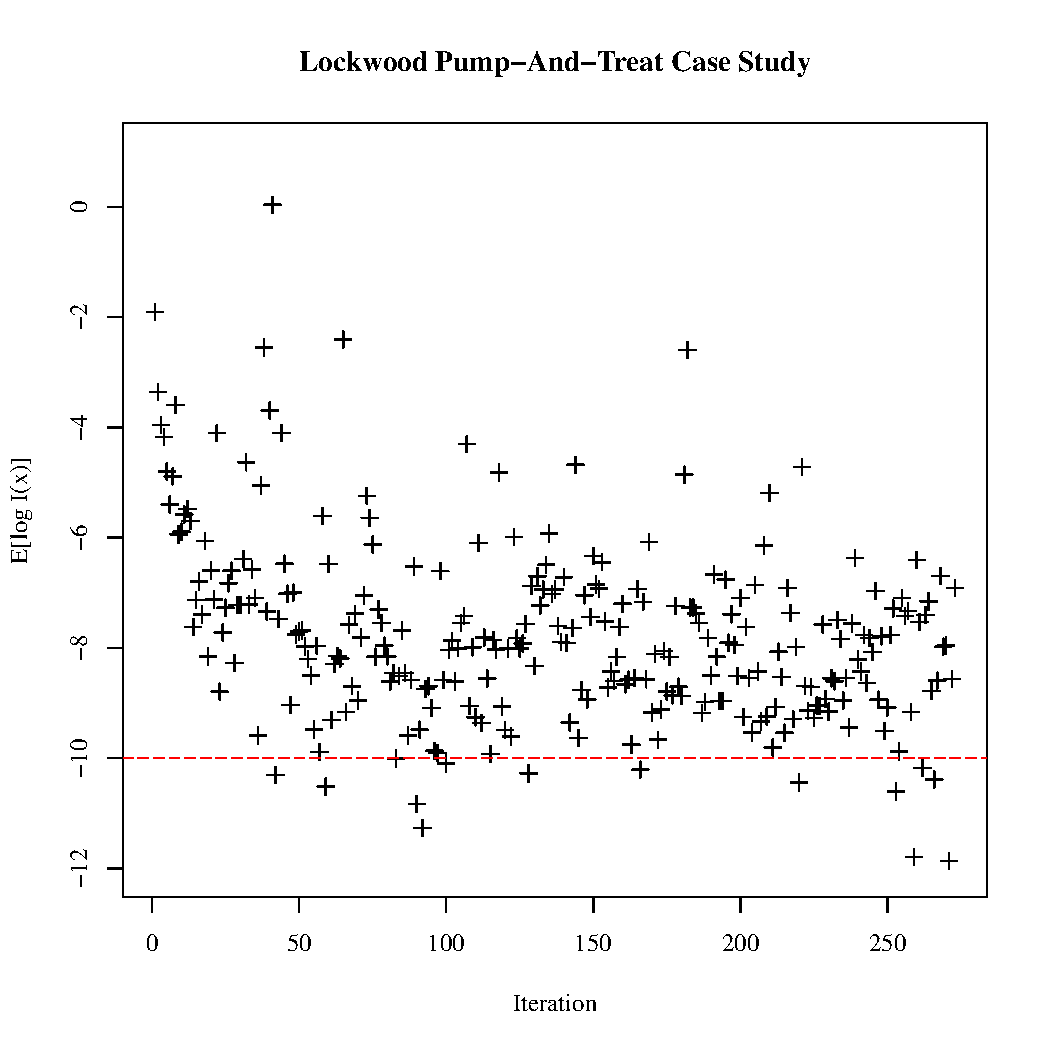
\includegraphics[width=0.32\textwidth]{./figures/introChartLock6Three20000Axis.pdf}
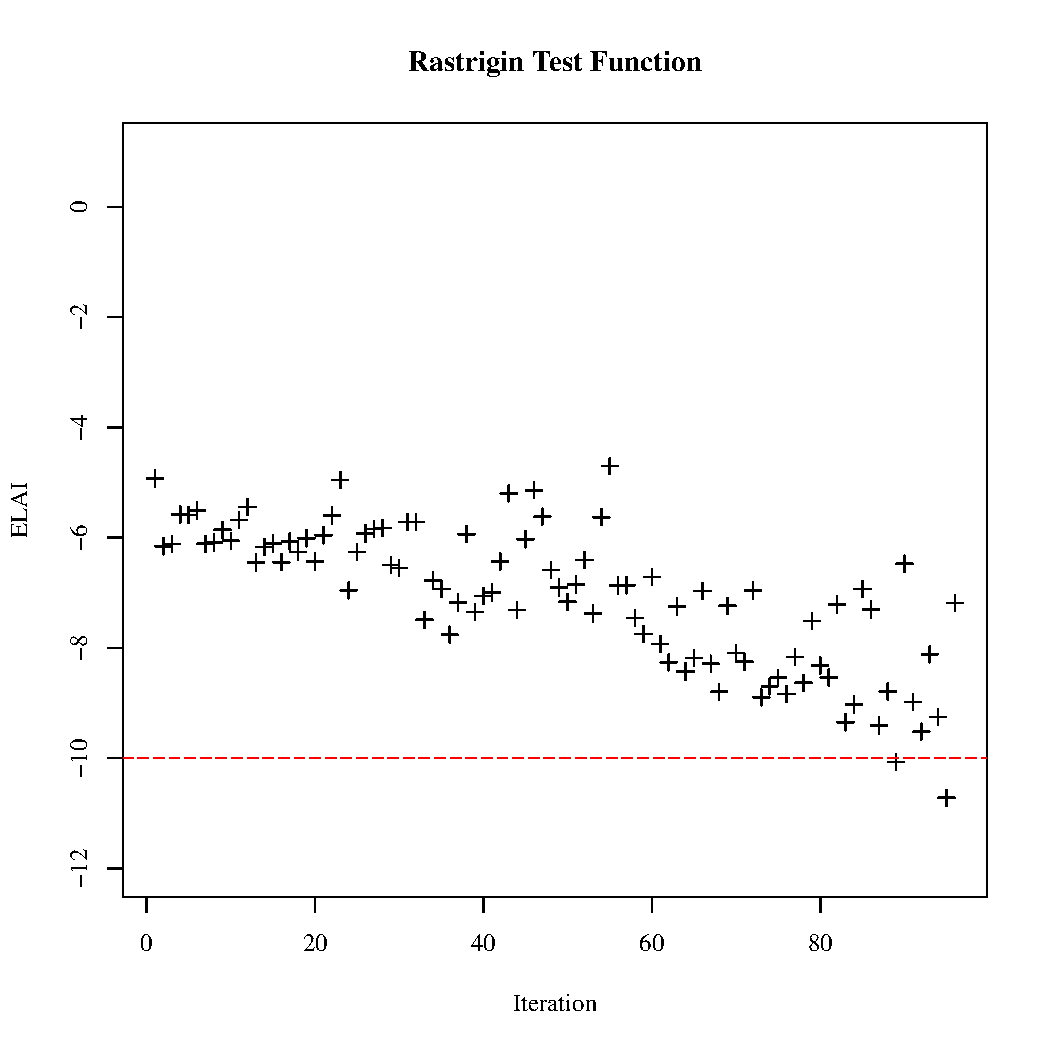
\includegraphics[width=0.32\textwidth]{./figures/introChartRastHardAxis.pdf}
\caption{
%
Three Expected Log-normal Approximation to the Improvement series (more details in Section~\ref{sec:examples}) plotted alongside an example convergence threshold value shown as a dashed line at -10.
}
\label{introFig}
\end{figure}
%
%

%%of the series value; of the values; shows; non-negative
%Because EI is strictly positive but decreasingly small,
%we find it more productive to work on the log scale, using a log-normal
%approximation to the improvement distribution to generate a more appropriate convergence criterion, as described in more
%detail in Section~3.2.
%%
%Figure~(\ref{introFig}) represents three series of the Expected
%Log-normal Approximation to the Improvement (ELAI) convergence criterion values from three
%different optimization problems that will be demonstrated later in
%this paper, where it will be shown that convergence is established near
%the end of each of these series.
%%as generated by 
%These three series demonstrate various ELAI convergence behaviors, and
%illustrate the difficulty in assessing convergence.  
%asymptotic properties of the; in more detail; improve
%In each panel the y-axis represents a monotone transformation of the basic EI criterion {\color{red}(i.e. ELI)} so as to benefit the asymptotic behavior of the improvement criterion's distribution, to be discussed further in Section {\color{red}XX}.

%of the series value; of the values; shows; non-negative
Because EI is strictly positive but decreasingly small,
we find it more productive to work on the log scale, using a log-normal
approximation to the improvement distribution to generate a more appropriate convergence criterion, as described in more
detail in Section~3.2.
%
Figure~(\ref{introFig}) represents three series of the Expected
Log-normal Approximation to the Improvement (ELAI) values from three
different optimization problems.
%
We will demonstrate later in this paper that convergence is established near the end of each of these series.
%as generated by 
These three series demonstrate the kind of diversity observed among various ELAI convergence behaviors, and illustrate the difficulty in assessing convergence.
%
In the left-most panel, optimization of the Rosenbrock test function 
results in a well-behaved series of ELAI values, demonstrating a case in 
which the simple threshold stopping rule can accurately identify convergence.
%as this series
However the center panel (the Lockwood problem) demonstrates a failure of 
the threshold stopping rule, as this ELAI series contains much more 
variance, and thus small ELAI values are observed quite regularly.
%for the remainder of the series.
In the Lockwood example a simple threshold stopping rule could falsely
claim convergence within the first 50 iterations of the algorithm.
%
The large variability in ELAI values with occasional large values indicates that 
the optimization routine sometimes briefly settles into a local minimum but is 
still exploring and is not yet convinced that it has found a global minimum.
%, additionally as the algorithm proceeds, several improvements of the objective function are discovered while ELI values repeatedly fall below the convergence threshold. %, all while the optimization routine continues to find several improved values of the objective function.
This optimization run appears to have converged only after the
larger ELAI values stop appearing and the variability has decreased.
%
Thus one might ask if a decrease in variability, or small variability,
is a necessary condition for convergence.  
%
The right-most panel (the Rastrigin test function) 
shows a case where convergence occurs by meeting the threshold level,
but where variability has increased, demonstrating that a decrease in
variability is not a necessary condition.

%
%

%
Since the Improvement function is itself random, attempting to 
set a lower threshold bound on the EI, without consideration of the underlying 
EI distribution through time, over-simplifies the dynamics of convergence
in this setting. 
%
Instead, we propose taking the perspective of Statistical
Process Control (SPC), where a stochastic series is monitored for 
consistency of the distribution of the most recently observed values.
In the next section, we review the statistical surrogate model approach and the use of EI for optimization.  In Section~\ref{sec:convergence}, we discuss our inspiration from SPC and how we construct our convergence chart.  Section~\ref{sec:examples} provides synthetic and real examples, and then we provide some conclusions in the final section. Throughout this paper we focus on minimization, as maximization can be obtained by minimizing the negative of the function.

\clearpage
%
%
\section{Gaussian Process Surrogate Model Optimization}
\label{sec:gp}
%
%

%
The primary motivation for the use of surrogate modeling in optimization is to manage a computationally challenging objective function with the use of a fast and relatively simple functional working model (i.e. the surrogate model) of the problem function. 
%
The surrogate model serves as an efficient tool for using function evaluations to infer the expected behavior of the objective function and thus determine where further optima may exist with minimal evaluation of the complex objective function itself.
%
Surrogate modeling is therefore useful for optimizing large computer simulation experiments, where each function evaluation may consume considerable computational resources, while the surrogate model can be evaluated quickly.
%
The standard surrogate model in the literature for analysis of computer experiments is a Gaussian process (GP) \citep{sacksDesign, santnerBook}. 
%that collenction
A GP is a stochastic process such that when evaluated at any finite collection of points, the collection follows a multivariate Gaussian distribution. 
%
A GP is defined by its mean function and its covariance function, with various standard formulations \citep{abrahamsenBook,steinBook}. 
%
Most formulations take advantage of a large degree of smoothness, reflecting a modeling assumption of smoothness in the output of the simulator, in that if the simulator is evaluated at two nearby inputs, then one expects the resulting outputs to be relatively close. 
%
A GP can interpolate, which can be useful for a deterministic simulator, or it can smooth, which has a number of practical advantages even for deterministic simulators \citep{gramacy2012}.

%GP surrogate modeling considers the objective function $f \sim \text{GP}\big(m(\bm{x}), ~C(\bm{x}, \bm{x}')\big)$, and thus aims to minimize the number of actual function evaluations by using the GP predictive surface to interpolate between function evaluations.
%learning
%The surrogate can be used to minimize the number of evaluations by accurately interpolating between function evaluations and contributing information about where further evaluations of the objective function may be most useful for finding new optima.
%Considering the goals of surrogate modeling in optimization, 
% In particular, GP surrogate models have become a standard tool for analysis of computer emulation experiments .
%
% GP models 
%Inference on such GP models seems to strike an equitable balance between relative ease of computation and efficient learning of the true objective function behavior.
%
%making them ideal candidates for use as surrogate models here.

%
%

%
%As with most popular optimization strategies for optimizing functions over a real domain, GP surrogate optimization can make use of the assumption of some cohesive smoothness of the objective function.
%
%This smoothness relates points close in space, with similar expectations for the objective value, providing the primary mechanism by which optimization may proceed in most numerical algorithms. 
%
%GPs can directly express this assumption of smoothness with the a'priori choice of an appropriate covariance function which smoothly relates points through their relative positions in the domain.
%
%The choice of a covariance function to represent a smooth objective function is the typical modeling choice for optimization in computer emulation \citep{santnerBook}, although theoretically GPs may accommodate many common covariance structures \citep{abrahamsenBook, steinBook}. 
%s smoothness based upon the particular 
% to relate  models require that the of smooth objective functions on $\mathbb{R}^p$.
%

%
%

%
In many cases the assumption of a globally smooth $f$ with a homogeneous uncertainty structure can provide an effective and parsimonious model.
%smoothness in the GP covariance structure may make sense for a wide variety of objective functions, it is desirable to 
However for the sake of providing a flexible surrogate model, it is desirable to have the ability to loosen these restrictions in cases when $f$ may have inherently sharp boundaries, or when numerical simulators have variable stability in portions of the domain. 
%
\cite{gpJasa} use the idea of allowing subpopulations of flexibility via a treed partitioning of the domain, fitting stationary GP surfaces to separate portions of $f$.
%
The domain is recursively sub-partitioned and separate hierarchically-linked GP models are fit within each sub-partition.
%
The partitioning scheme is fit via a reversible jump MCMC algorithm, jumping between models with differing partitioning schemes, and averaging over the full parameter space to provide smooth predictions except where the data call for a discontinuous prediction.
%
Partitioning the domain in this way allows parsimonious surrogate models in simple objective function cases and quite flexible surrogate models when the objective function displays complex behavior. 
%
For further explanation of partitioned Gaussian process models, as well as notes on implementing such models in R, see the R package \verb tgp  \citep{tgp, tgp2}.  
%
Because many of the objective functions of interest are not well modeled by a stationary GP, we use treed GPs as our surrogate models in this paper, but our approach is easily adaptable to a wide variety of surrogate models.

%       In many cases the assumption of a smooth $f$ with a homogeneous uncertainty structure can provide an effective and parsimonious model.
%       %
%       However for the sake of providing a flexible surrogate model, it is desirable to have the ability to loosen these restrictions in cases when $f$ looks more like the Grand Canyon, as opposed to the Great Plains.     
%       %objective landscape
%       Gramacy and Lee \cite{gpJasa} introduce the idea of allowing this flexibility via a treed partitioning of the domain.
%       %
%       This allows separately stationary GP surfaces to fit separately stationary portions of $f$.
%       %
%       For further explanation of partitioned Gaussian process models as well as notes on implementing such models in R, see the R package \verb tgp  \cite{tgp, tgp2}.

% surrogate models should compute in a relatively short amount of time as compared with the objective function quick to compute, and should quickly learn the behavior of the 
% 
% , based on the available data from the objective function. and thus aid use each evaluation of the objective function as a  
% It is of primary interest that the surrogate model can  efficiently incorporate each function evaluation 
% 
% %
% The primary idea behind surrogate modeling is to manage computationally difficult objective functions by constructing a functional working model (i.e. a surrogate model) of the true objective function, to be optimized, to represent as much about the objective function as our current data allows.
% %
% Surrogate modeling is a useful tool for application to large computationally expensive 
% %
% The primary role of surrogate modeling is to quickly and as accurately as possible construct a    optimization the primary 

%
%
% \begin{itemize}
% % \item {\color{red} *Everybody uses GP, bunch of cites}
% %
% % \item Gaussian process surrogate modeling has become a standard tool for analysis of computer emulation experiments \cite{sacksDesign, santnerBook} as well as many 
% %
% % \item other applications in which an a'priori assumption of smoothness is useful .
% %
% % \item For the sake of optimization, the assertion of a smooth objective function, $f$, serves as the basis for most efficient searching algorithms.%, as is explicitly the case with GP.
% %
% % \item In the case of GP surrogate modeling, the Gaussian process theory can explicitly express this desire for smoothness through the a'priori choice of a covariance function with the desired smoothness properties.
% %
% % \item Although smoothness is key to search, and 
% %  
% \item For the sake of optimization practically all opt we only have a hope of efficiently searching $f$ if we assume that $f$ provides a reasonably smooth, otherwise optimization by any method is practically infeasible.
% %
% \item However it is not 
% 
% %
% \item \cite{gpJasa, tgp, tgp2}
% %
% \item {\color{red} *Expand Treed Partitioning}
% %
% \item For additional modeling details, including loosening the assumption of global stationarity, and details about implementing GP models in the context of numerical optimization see the R package \verb tgp ~as well as the associated vignettes \cite{tgp, tgp2}.
% \end{itemize}


% If we have any hope of finding optima of a function, $f$, we impose the condition that $f$ provides a reasonably smooth mapping for relating points in the domain, $\bm{x}$, to response values, $z(\bm{x})$.
% optimization of functions over $\mathbb{R}^p$
% %
% GP surrogates, as with many optimization strategies for objective function on $\mathbb{R}^p$, rely upon some sense of cohesive smoothness of the objective function, which relates points close in space with similar expectations for the objective value.

% {\color{red} *Everybody uses GP, bunch of cites}
% 
% %
% For more details on the theoretical foundations of Gaussian processes in computer experiments see \cite{santnerBook}.
% %
% If we have any hope of finding optima of a function, $f$, we impose the condition that $f$ provides a reasonably smooth mapping for relating points in the domain, $\bm{x}$, to response values, $z(\bm{x})$.
% %\text{\textbf{Z}}; $\big($i.e.~\big)$; \text{Z}
% The $z(\bm{x})$ are assumed to be particular realizations of an infinitely dimensional generalization of the multivariate normal distribution, $f \sim \text{GP}(m,~K)$, and thus jointly any set of such realizations, $z(\bm{x})$, jointly follow a multivariate normal distribution.
% %
% As part of the GP model specification, we specify the mean function as a linear combination of simple basis functions, $m=\bm{\beta}^\intercal \text{\textbf{f($\bm{x}
% $)}}$, and we describe the covariance structure, among the dimensions of the $z(\bm{x})$, through specification of a covariance function, $K(\bm{x}, \bm{x}')$.
% %
% By specifying a homogeneous covariance function, we thus model the relationship between $||\bm{x}-\bm{x}'||$ with the correlation structure that we expect to see when jointly considering two such realizations of the GP. 
% %
% The following exponential power family provides an example of a reasonable choice of $K(\bm{x}, \bm{x}')$, under the assumption of a reasonably well behaved $f$,
% %
% \begin{equation}
% K(\bm{x}, ~\bm{x}') = \sigma^2\exp\left\{ -\frac{||\bm{x}-\bm{x}'||^p}{d} \right\}.
% \label{corrFunc}
% \end{equation} 
% %
% Specifying conjugate priors for $\bm{\beta}$ and $\sigma^2$ yields a straightforward Gibbs sampling posterior inferential setting with the exception of the covariance structure parameters requiring Metropolis-Hastings MCMC sampling.


%
%
\subsection{Expected Improvement}
%
%

%
%The EI criterion has been used \cite{tgp2}, \cite{taddyOpt} to identify candidate points that have a strong {\it possibility of encountering new minima}.
%when applied to a single candidate point has
%The EI criterion predicts how much smaller a minimum is likely to be found at a potential new minimum location based on the predictive surrogate model.  EI is built upon the improvement function \citep{jonesEIOpt}:
%(i.e. a smaller value of the objective function) 
The EI criterion predicts how likely a new minimum is to be observed, at new locations of the domain, based upon the predictive distribution of the surrogate model.  
%
EI is built upon the improvement function \citep{jonesEIOpt}:
%
%The improvement function takes the following form,
\begin{equation}
\ix~=~ \max \Big\{ \big(f_{min} - f(\bm{x})\big), ~0 \Big\},
\label{ix}
\end{equation}
%
where $f_{min}$ is the smallest function value observed so far.  
%
EI is the expectation of the improvement function with respect to the posterior predictive distribution of the surrogate model, $\Eix$.
%
EI rewards candidates both for having a low predictive mean, as well as high uncertainty (where the function has not been sufficiently explored).
%
By definition the improvement function is always non-negative and the GP posterior predictive $\Eix$ is strictly positive.
%
The EI criterion is available in closed form for a stationary GP.
%
For other models the EI criterion can be quickly estimated using Monte Carlo posterior predictive samples at given candidate locations.

\clearpage
%
%
\subsection{Optimization Procedure}
%
%

%
%
\begin{wrapfigure}{r}{0.5\textwidth}
	\vspace{-0.8cm}
        %\vspace{-1.6cm}
        %\vspace{-2.5cm}
	%\vspace{-3.5cm}
        \singlespacing
        \caption{Optimization Procedure}
        \begin{itemize}
        \item[1)] Collect an initial set, $\bm{X}$.
        \item[2)] Compute $f(\bm{X})$.
        \item[3)] Fit surrogate based on evaluations of $f$.
        \item[4)] Collect a candidate set, $\tilde{\bm{X}}$.
        %\item[5)] Compute $\Eix$ among $\tilde{\bm{X}}$.$\E{\text{I}(\tilde{\bm{x}_i}})$
        \item[5)] Compute EI among $\tilde{\bm{X}}$
        %\item[6)] Add $\tilde{\bm{x}_i}$ yielding largest $\Eix$ to $\bm{X}$.
        \item[6)] Add $\argmax_{\tilde{\bm{x}_i}} \E{\text{I}(\tilde{\bm{x}_i})}$ to $\bm{X}$.
        \item[7)] Check convergence.
        \item[8)] If converged exit. Otherwise go to 2).
        \end{itemize}
        \doublespacing
        %\vspace{-0.85cm}
        \label{procedure}
\end{wrapfigure}
%
% us with a
Optimization can be viewed as a sequential design process, where locations are selected for evaluation on the basis of how likely they are to decrease the objective function, i.e., based on the EI.
%The idea for optimization, in this context, is to only evaluate the objective function at locations that have a good chance of providing a new minimum. 
%I need a handle
Optimization begins by initially collecting a set, $\bm{X}$, of locations to evaluate the true function, $f$, to gather a basic impression of $f$.
% (\ref{gpModel})
A statistical surrogate model is then fitted with $f(\bm{X})$ as observations of the true function.
%EI randomly
Using the surrogate model, a set of candidate points, $\tilde{\bm{X}}$, are selected from the domain and the EI criterion is calculated among these points.
%
The candidate point that has the highest EI is then chosen as the
%
best candidate for a new minimum and thus, it is added to $\bm{X}$.
% (\ref{gpModel})
The objective function is evaluated at this new location and the surrogate model is refit based on the updated $f(\bm{X})$.
%
The optimization procedure carries on in this way until convergence.  The key contribution of this paper is an automated method for checking convergence, which we develop in the next section. 

%$~$\\
%\vspace{-0.6cm}
%
%
\section{EWMA Convergence Chart}
\label{sec:convergence}
%
%

%
%
\subsection{Statistical Process Control}
%
%

%
In Shewhart's seminal book \citep{shewhartBook} on the topic of control in manufacturing, Shewhart explains that a phenomenon is said to be in control when, ``through the use of past experience, we can predict, at least within limits, how the phenomenon may be expected to vary in the future.''
%, accounting not only for the the expected variability  not only consider particular values of the EI criterion, but it ( expected center, spread, and )
This notion provides an instructive framework for thinking about convergence because it offers a natural way to consider the distributional characteristics of the EI as a proper random variable. 
% of that statistic.
In its most simplified form, SPC considers an approximation of a statistic's sampling distribution as repeated sampling occurs in time.
Thus Shewhart can express his idea of control as the expected behavior of random observations from this sampling distribution.
% from some data generating mechanism,
For example, an $\bar x$-chart tracks the mean of repeated samples (all of size $n$) through time so as to expect the arrival of each subsequent mean in accordance with the known or estimated sampling distribution for the mean, $\bar{x}_j \sim N\left(\mu, \frac{\sigma^2}{n}\right)$.   
%
%Shewhart expresses his idea of control as the expected behavior of random observations from the sampling distribution of interest.
%easily
By considering confidence intervals on this sampling distribution we can draw explicit boundaries (i.e. control limits) to identify when the process is in control and when it is not.
%
Observations violating our expectations (falling outside of the control limits) indicate an out-of-control state.
%it is of primary importance to use the data carefully to form accurate approximations of these values, thus establishing a standard for control
Since neither $\mu$ nor $\sigma^2$ are typically known, it is common to collect an initial set of data from which point estimates of $\mu$ and $\sigma^2$ may establish an initial standard for control which is further refined as the process proceeds.
%
Furthermore, this logic relies upon the typical asymptotic results of the central limit theorem (CLT), and care should be taken to verify the relevant assumptions required.

%
It is important to note that we are not performing traditional SPC in this context, the EI criterion will be stochastically decreasing as an optimization routine proceeds.  
%
Only when convergence is reached will the EI series look approximately like an in-control process.  
%
Thus our perspective is completely reversed from the traditional SPC approach---we start with a process that is out of control, and we determine convergence when the process stabilizes and becomes locally in control.  
%
An alternative way to think about our approach is to consider performing SPC backwards in time on our EI series.  
%
Starting from the most recent EI observations and looking back, we declare convergence if the process starts in control and then becomes out of control.  
%
This pattern generally appears only when the optimization has progressed and reached a local mode.  
%
If the optimization were still proceeding, then the EI would still be decreasing and the final section would not appear in control.

%
%
\subsection{Expected Log-normal Approximation to the Improvement (ELAI)}
%
%

%
For the sake of obtaining a robust convergence criterion to track via SPC, it is important to carefully consider properties of the improvement distributions which generate the EI values.
%
% Ultimately, the distribution of the EI is asymptotically normal, but the characteristics of the improvement distribution, as convergence approaches, complicate these asymptotics. 
%
The improvement criterion is strictly positive but decreasingly small, thus the improvement distribution is often strongly right skewed, in which case, the EI is far from normal.
%
Additionally, this right skew becomes exaggerated as convergence approaches, due to the decreasing trend in the EI criterion.
%% distribution will always struggle to capture the resulting EI distribution.
Together these characteristics of the improvement distribution give the EI criterion inconsistent behavior for tracking convergence via a typical $\bar x$-chart. 
 
%
%

%log improvement
These issues naturally suggest releasing the bound at 0 by modeling transformations of the improvement, rather than directly considering the improvement distribution on its own.
%
One of the simplest of the many possible helpful transformations in this case would consider the log of the improvement distribution. 
%
However due to the MCMC sample-based implementation of the Gaussian process, and the desire for a large number of samples from the improvement distribution, it is not uncommon to obtain at least one sample that is computationally indistinguishable from 0 in double precision.
%
Thus simply taking the log of the improvement samples can result in numerical failure, particularly as convergence approaches, even though the quantities are theoretically strictly positive.
%
Despite this numerical inconvenience, the distribution of the improvement samples is often very well approximated by the log-normal distribution. 

%
%

%
We avoid the numerical issues by using a model-based approximation. 
%
With the desire to model $\mathbb{E}\left[~\log\text{I}~\right] \approxdist N\left(\mu, \frac{\sigma^2}{n}\right)$, we switch to a log-normal perspective.   
%
Recall that if a random variable \mbox{$X\sim Log$-$N(\theta, \phi)$,} then another random variable $Y=\log(X)$ is distributed $Y\sim N(\theta, \phi)$.
%{\color{red}cite}
Furthermore, if $\omega$ and $\psi$ are, respectively, the mean and variance of a log-normal sample, then the mean, $\theta$, and variance, $\phi$, of the associated normal distribution are given by the following relation.
%
\begin{eqnarray}
\theta = \log\left( \frac{\omega^2}{\sqrt{\psi+\omega^2}} \right) &~&  \phi = \log\bigg( 1+ \frac{\psi}{\omega^2} \bigg).
\label{lnRelate}
\end{eqnarray}
%
Using this relation we do not need to transform any of the improvement samples.
%
We compute the empirical mean and variance of the unaltered, approximately log-normal, improvement samples, then use relation (\ref{lnRelate}) to directly compute $\psi$ as the Expectation under the Log-normal Approximation to the Improvement (ELAI).
%Considering that the log improvement has reduced right skew, for the sake of improved asymptotics of the; of the $\E{\log\text{I}}$ distribution enjoys improved asymptotics
The ELAI value is useful for assessing convergence because of the reduced right skew of the log of the posterior predictive improvement distribution.
%
Additionally, the ELAI serves as a computationally robust approximation of the $\E{\log\text{I}}$ under reasonable log-normality of the improvements.
%approximately
Furthermore, both the $\E{\log\text{I}}$ and ELAI are distributed approximately normally in repeated sampling.
%
This construction allows for more consistent and accurate use of the fundamental theory on which our SPC perspective depends.

%improvement provides robust asymptotics for the normality of the distribution of the $\E{\log\text{I}}$, even as convergence approaches the ELAI provides a good approximation for this value.
%{\color{red} ELAI}
% The ELAI provides a good approximation for 

%
%
\subsection{Exponentially Weighted Moving Average}
%
%

%
The Exponentially Weighted Moving Average (EWMA) control chart \citep{ewmaPaper, qccPack} elaborates on Shewhart's original notion of control by viewing the repeated sampling process in the context of a moving average smoothing of series data. %, rather than assuming a constant long run average, as in the $\bar x$-chart.    
%Principally provide particularly robust solutions to be expected for convergence in this setting.
Pre-convergence ELAI evaluations tend to be variable and overall decreasing, and so do not necessarily share distributional consistency among all observed values.  
%
Thus a weighted series perspective was chosen to follow the moving average of the most recent ELAI observations while still smoothing with some memory of older evaluations.
%stochastically slides into convergence, a series perspective is appropriate here; in particular the EWMA perspective has shown to be well suited for tracking the progression of means that are subject to subtle drifting processes \cite{adaptEWMA, ?}. %, just as displayed by the ELAI criterion upon convergence.
%
EWMA achieves this robust smoothing behavior, relative to shifting means, by assigning exponentially decreasing weights to successive points in a rolling average among all of the points of the series. 
%
Thus the EWMA can emphasize recent observations and shift the focus of the moving average to the most recent information while still providing shrinkage towards the global mean of the series.

%
%

%
If $Y_i$ is the current ELAI value, and $Z_i$ is the EWMA statistic associated with this current value, then the initial value $Z_0$ is set to $Y_0$ and for $i\in\{1, 2, 3, ...\}$ the EWMA statistic is expressed as,
%
\begin{equation}
Z_i=\lambda Y_i+(1-\lambda)Z_{i-1}.
\label{ewmaStat}
\end{equation}
%
Above, $\lambda$ is a smoothing parameter that defines the weight $\left( \text{i.e. }0<\lambda\le1\right)$ assigned to the most recent observation, $Y_i$.
%Eq. (\ref{ewmaStat})
The recursive expression of the statistic ensures that all subsequent weights geometrically decrease as they move back through the series.

% \clearpage
%
% \vspace{-0.8cm}
%
\cite{boxBook} describes typical values of $\lambda$ in the range \mbox{$0.1\le\lambda\le0.3$}, with large values of $\lambda$ producing a more myoptic weighting scheme. 
%
Furthermore \cite{boxBook} also describes a method for computing optimal choices of $\lambda$ by minimizing the sum of squared forecasting deviations ($S_\lambda$).
%
For each new observation, 
\begin{equation}
\hat\lambda=\argmin_{\lambda\in(0,1]}\bigg(\sum_i \Big(Y_i-Z_{i-1}(\lambda)\Big)^2\bigg).
\end{equation}

%
Through this analysis of $S_\lambda$, as seen in Figure~(\ref{bestL}), it is evident that EWMA charts can be very robust to reasonable choices of $\lambda$, due to the small first and second derivatives of $S_\lambda$ for a large range of sub-optimal choices of $\lambda$ around $\hat\lambda$. % as seen in Figure~(\ref{bestL}).
%
In fact, Figure~(\ref{bestL}) shows that for \mbox{$\lambda\in[0.2, 0.6]$,} $S_\lambda$ stays within 10\% of its the minimum possible value.


%, with a default value of $\lambda$ around $0.2$, as described by \cite{boxBook}.
% %
% % Large values of $\lambda$ assign more weight to recent observations in the series, allowing for a more flexible fit for unstable series.
% %
% % However, the choice of a large $\lambda$ may over-fit the $Z_i$ to noise in the $Y_i$.
% %
% It is thus desirable to choose to the smallest $\lambda$ which still provides good forecasts of future
% observations in the series.
% %\cite[p. 87]{boxBook}  %Box et al. (1997, p. 87)
% \cite{boxBook} explains how to choose an optimal value for $\lambda$ by choosing the $\hat\lambda$ which minimizes the sum of squared forecasting deviations ($S_\lambda$) for each new observation.
% %curvature

%
%
\begin{wrapfigure}{r}{0.41\textwidth}
%\vspace{-0.8cm}
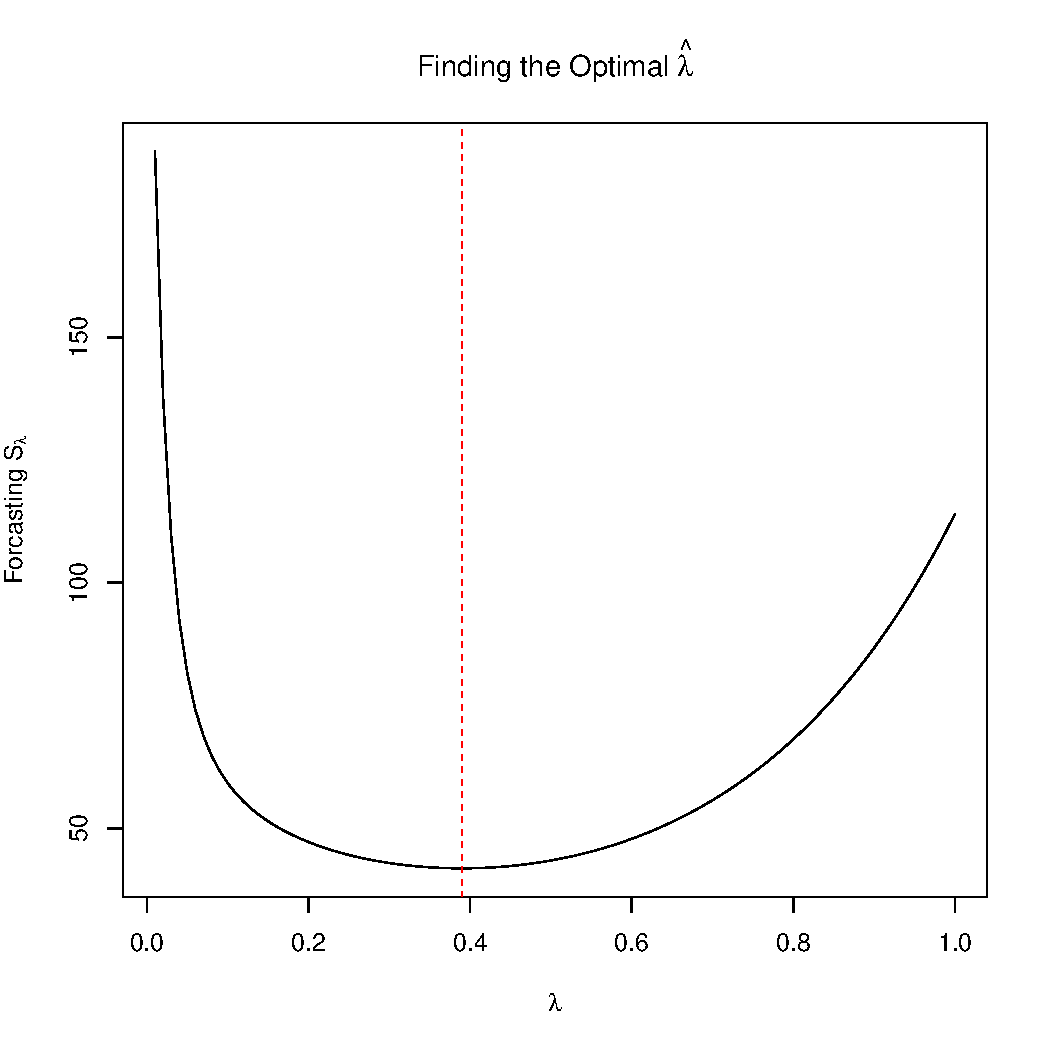
\includegraphics[width=0.4\textwidth]{./figures/ssRastHardOpt.pdf}
\caption{ $S_\lambda$ as calculated for ELAI values derived from optimization of the Rastrigin test function. $\hat\lambda$ is shown by the vertical dashed line. }
\label{bestL}
\end{wrapfigure}
%
%

%
It is interesting to note that for the example series used in Figure~(\ref{bestL}), the optimal \mbox{$\hat \lambda\approx$\rastLamb} exceeds the recommended upper limit of 0.3 for $\lambda$. 
%
Discrepancies between the optimal values of $\lambda$ chosen here, and those typically chosen can be naturally attributed to the differing context in which we apply EWMA, as compared to the typical SPC application. 
%which obviously falls outside of the standard values for $\lambda$ mentioned above.
%would begin with starts; new
The typical use of EWMA in SPC begins with the premise of a relatively stable (in-control) series and attempts to identify out-of-control observations which would indicate some change in the data generating process.
%
However our use of EWMA to identify convergence begins with an out-of-control series and we wish to identify when the series falls into control (i.e. convergence).
%
As a result, ELAI values for tracking convergence are inherently less stable than typical SPC applications.
%
These larger values of $\lambda$ allow the EWMA to track the movement of ELAI values from pre-convergence into convergence.
%% in the context of identifying convergence.
% Due to the decreased stability of the series, in this context, the optimal forecasting $\hat\lambda$ may often fall above the traditionally recommended upper limit for $\lambda$, in-order to better follow the more active moving averages inherent to the unstable pre-convergence series. 
%
In this context we want to reiterate that while it is useful to borrow the EWMA machinery often used in SPC, we are approaching the whole process backwards, in that we are starting with an ``out of control'' process and waiting to see when it settles down into control, and thus our approach should be viewed as SPC-inspired rather than a formal application of SPC.
% but the ultimate analysis of the data should not explicitly be considered SPC, as the perspective of the data does not fully align with that of SPC.

%
%

%Identifying convergence relies upon carefully defining the control limits on the EWMAstatistic.
Identifying convergence in this setting, now requires the computation of control limits on the EWMA statistic. %comparisonrelies upon the relative positions of the EWMA statistic and the control limits on the EWMA statistic.
%
As in the simplified $\bar x$-chart, defining the control limits for the EWMA setting amounts to considering an interval on the sampling distribution of interest.
%, under the assumptions that the $Y_i$ arrive as $i.i.d.$ samples
In the EWMA case we are interested in the sampling distribution of the $Z_i$.
%, Lucas and Saccucci \cite{ewmaPaper}  show,
Assuming that the $Y_i$ are $i.i.d.$ then \cite{ewmaPaper} show that we can write $\sigma^2_{Z_i}$ in terms of $\sigma^2_{Y}$. 
%
\begin{equation}
\sigma^2_{Z_i} = \sigma^2_{Y}\left(\frac{\lambda}{2-\lambda}\right)\left[1-(1-\lambda)^{2i}\right]
\end{equation}
%\substack{i.i.d.\\\sim}
Thus if $Y_i \stackrel{i.i.d.}{\sim} N\left(\mu, \frac{\sigma^2}{n}\right)$, then the sampling distribution for $Z_i$ is $Z_i \sim N\left(\mu, \sigma^2_{Z_i}\right)$.
%
Furthermore by choosing a confidence level through choice of a constant $c$, the control limits based on this sampling distribution are seen in Eq. (\ref{EWMACL}).% follow on the next page.
%
%
%
\begin{equation}
\text{CL}_i = \mu \pm c \sigma_{Z_i}
=  \mu \pm c ~ \frac{\sigma}{\sqrt{n}}~\sqrt{\left(\frac{\lambda}{2-\lambda}\right)\left[1-(1-\lambda)^{2i}\right]}
\label{EWMACL}
\end{equation}
%
%

%
Notice that since $\sigma^2_{Z_i}$ has a dependence on $i$, the control limits do as well.
%the focusing effect of EWMA. % this focusing effect.\frac{\sigma}{\sqrt{n}}~
Looking back through the series brings us away from the focus of the moving average, at $i$, and thus the control limits widen until the limiting case as, $i\rightarrow\infty$, where the control limits are defined by $\mu \pm c ~ \sqrt{\frac{\lambda\sigma^2}{(2-\lambda)n}}$.
%traversing backwards through the series resulting directly from the geometrically decreasing weights.

%
Our aim in applying the EWMA framework in this context is to recognize the fundamental notion of control that EWMA enforces in the newly arriving EI values, as optimization proceeds.
%(and furthermore the ELAI distribution as well
Convergence often arrises as a subtle shift of the EI distribution into place.
%
In this context a more traditional $\bar x$ chart will often overlook convergence as a subtle random fluctuation, when in fact it is often this subtle signal that we aim to pick-up.
%designed with the recognition of subtlely shifting means in mind {(\color{red}cite)}.
EWMA is amoung the better techniques for recognizing such subtlely shifting means{\color{red}\cite{aerne1991trend, zou2009compare}}, while maintaining the capability to detect abrupt shifts in mean.
%
As convergence approaches the newly arriving $Y_i$ begin to fit into the $i.i.d.$ EWMA framework and the $Z_i$ increasingly begin to fall within the EWMA control limits.
%
EWMA's recognition of such a controlled region in the newly arriving ELAI values, indicates the notion of distributional consistency that is neccisary for defining convergence for stochastic measures of convergence, such as EI. 


% %
% At first glance it is not clear that the $Y_i$ are in fact $i.i.d.$
% %
% Indeed the early iterations of the convergence processes seen in Figure (\ref{introFig}) certainly do not display $i.i.d.$ $Y_i$. 
% %
% However as the series approaches convergence, the $Y_i$ eventually do enter a state of control, see for example Figure~(\ref{fig:rosenbrock}).
% %
% For these $Y_i$ at convergence, an $i.i.d.$ approximation is reasonable.
% %
% The realization of such a controlled region of the series defines the notion of consistency that allows for the identification of convergence. 

%
%
\subsection{The Control Window}
%
%

% for accurate identification of convergence is the introduction of a so called
%the distributional consistency we use to identify convergence
% that is necessary
The final structural feature of the EWMA convergence chart for identifying convergence is the so called {\it control window}.
%is a window containing
The control window contains a fixed number, $w$, of the most recently observed $Y_i$.
%The idea being, o
Only information from the $w$ points currently residing inside the control window is used to calculate the control limits, however to assess convergence the EWMA statistic is computed for all $Y_i$ values.
%
Initially, the convergence algorithm is allowed to fill the control window by collecting an initial set of $w$ observations of the $Y_i$.
%
As new observations arrive, the oldest $Y_i$ value is removed from the control window, thus allowing for the inclusion of a new $Y_i$.

%
%

%
The purpose of the control window is two-fold.
% examination
First, it serves to dichotomize the series for evaluating subsets of the $Y_i$ for distributional consistency.
% convergence
Second, it offers a structural way for basing the standard for consistency (i.e., the control limits) only on the most recent and relevant information in the series. 
%
%It is important to draw 
%This is important due to the subtle way in which ELAI values slide to convergence.

%
%

% {\color{red}
% %The size of this window is left up to the discretion of user,.
% The size, $w$, of the control window is an important parameter for correctly identifying convergence.
%
The size of the control window, $w$, may vary from problem to problem based on the difficulty of optimization in each case. %; ultimately the choice of $w$ is left as tuning parameter of the system.
%
A reasonable way of choosing $w$ is to consider the number of observations necessary to establish a standard of control. % in a similarly as a kind of sample size calculation. % with respect to the objective function at hand.
%
In this setting $w$ is a kind of sample size, and as such the choice of $w$ will naturally increase as the variability in the ELAI series increases.
%
% The choice of $w$ will naturally increase as the variability in the ELAI series increases. % difficulty of the optimization problem increases.
%
%For example, if the objective function is in many dimensions, the choice of $w$ will neccisarily increase to allow the surrogate model to gather a proportional amount of information about $f$.  
%
%The choice of a conservatively large $w$ consistently provides a better identification of convergence, with large $w$ representing idealistic large sample sizes, and small $w$ correctly identifying convergence well only for well-behaved functions, with small search domains.
%the size of the control window may lead to premature identification of convergence, however if $w$ is too large, we compute 
%as $w$ may be viewed in the context of 
%However, j(i.e. the cost of overadditional sampling)
Just as in other sample size calculations, the choice of an optimal $w$ must consider the cost of poor inference (premature identification of convergence) associated with underestimating $w$, against the cost of over sampling (continuing to sample after convergence has occurred) associated with overestimating $w$.
%
Providing a default choice of $w$ is somewhat arbitrary without careful analysis of the particulars of the objective function behavior and the costs of each successive objective function evaluation. %, however as a recommendation for starting this analysis, our experience suggests considering $w\ge15p$ as a lower bound. %rule of thumb.
%

%
For the purpose of exploring the behavior of $w$ in examples presented here, we use the following proceedure for educating the choice of $w$.
We hand tune $w$ for two informative known example functions (i.e. Rosebrock and Rastrigin).
From exploration of $w$ in known examples, it is clear that $w$ increases directly with ELAI variance.
Furthermore, if one considers the form of sample size calculations based on {\color{red}classical power analysis, sample size increases directly proportional with the sample variance.}
Thus we linearly extrapolate the choice of $w$ for the Lockwood case study based on a defalt starting value of 30 (based on sampling conventions) with a slope term structured to make use of the proportionality of $w$ with the observed ELAI variance, $\hat w=\frac{\Delta w}{\Delta \text{V(ELAI)}}\hat v+30$.
Further exploration of the exact form of an estimator of $w$ is left to be discovered, although the connection of $w$ with sample size calculations is a promising line of research in itself.



% Assuming approximate proportionality between $w$ and the ELAI variance, $v$, we extrapolate the choice of $w$ for the Lockwood case study based on the log-linear relationship $\log(w)=\beta_1 v+\beta_0$.
% It then follows that the estimates for the $\bm{\beta}$ are $\hat\beta_1=\frac{\Delta \log(\hat w)}{\Delta \hat v}$, and $\hat \beta_0 = \log(\hat w)-\hat\beta_1 \hat v$. 
% Further exploration of the exact form of an estimator of $w$ is left to be discovered, although this quick log-linear prediction is a promising line of research in itself, as it preserves the expected portionality between $w$ and the ELAI variance as implied by power analysis. 

% the consideration of $w$ as a kind of sample size suggested 
% We then extrapolate further choices of $w$ based on observed ELAI varianceLockwood pump and Treat based on the observed ELAI variances. 
% 
% in  for a third unknown example function.
% From analysis of the behavior of $w$ in know examples it is clear that $w$ increases directly with ELAI variance.
% based on observed ELAI variance.
% 
% 
% Furthermore if one considers that form of sample size calculations based on classical power analysis, sample size increases proportionally  the consideration of $w$ as a kind of sample size suggested 
% , and extrapolate the choice of $w$ from these known cases to the unknown case of the Lockwood pump and treat problem based on the rough assumptions that $w\propto Var(ELAI)$ and that relationship is roughly linear for large $Var(ELAI)$.


% {\color{red}
% $w\propto Var(ELAI)$
% % %
% % This recommendation considers the dimensionality, $p$, of the objective function and represents the prior assertion that premature identification of convergence is a worse error than computing extraneous objective function evaluations. 
% 
% %
% %
% %however the goal of identifying convergence is to 
% %
% % Choosing the correct value of $w$ presents an interesting decision problem since underestimating the size of the control window may lead to premature identification of convergence, however if $w$ is too large, we compute unnecessary objective function evaluations.
% %
% %
% 
% %
% For example, if the objective function must be searched over a large domain, particularly in many dimensions, optimization will naturally take many function evaluations to gather adequate information to reflect confident identification of convergence.
% %
% Thus the EI criterion, and by extension the ELAI criterion, may display high variance, associated with high uncertainty, as well as be slow to decrease in mean value from the initial state of pre-convergence into convergence.
% %
% Jointly the high ELAI variance and the slow decreasing mean ELAI value may make it hard to identify convergence; in these cases large values of $w$ are required to discern this relatively slight signal in the context of increased noise.
% %
% Similar effects may be observed for highly multimodal objective functions, as the regular discovery of new modes will increase the variance of the ELAI criterion, and disguise any decreasing mean value among the noise inherent to the search of such functions.
% 
% %
% %
% % %adequate algorithm willay EI criterion may commonly be slow to learn the  decrease from  display a large variance among among function evaluations, 
% % % Because $w$ may vary from problem to problem it is ultimately left as a tuning parameter of the system.
% % %
% % 
% % %
% % As a general trend, {\color{blue}harder} optimization problems require larger values of $w$ since the EI criterion follows a less structured decreasing pattern as new modes are discovered at irregular patterns.
% %
% %
% 
% %
% By contrast, strongly unimodal functions will enjoy a relatively fast decrease in ELAI in the presence of relatively small variability.
% %
% This higher signal-to-noise ratio makes for easier identification of convergence, and thus allows for a smaller choice of $w$. % to notice a move of the ELAI criterion into convergence.
% %
% However if $w$ is chosen to be too small, the algorithm may be over eager to claim convergence and the recommendation of $w\ge15p$ is particularly apt here to guard against false identification of convergence.   
% }

%
%

% {\color{red}
% %
% Choosing the correct value of $w$ presents an interesting decision problem since underestimating the size of the control window may lead to premature convergence, but if $w$ is too large, we compute unnecessary objective function evaluations.
% %It is t
% Thus it may be important to consider these two opposing forces when choosing an appropriate value for $w$.
% %
% I recommend conservatively large values for $w$ because I regard premature convergence to be a greater problem than extraneous function evaluations.
% %
% As a default value $w=30$ has provided me a reasonable starting point for further analysis.
% %
% I have found that choosing $w$ based on the value of $\lambda$ seems to be an efficient way of tuning $w$.
% %
% As a general trend, the larger the value of $\lambda$, the more fluctuation present in the EWMA statistic.
% %% the fluctuations in the EWMA statistic. %Conversely for small $\lambda$, smaller values of $w$ are acceptable. are necessary allow averages over more elements of he  to  average out ; fluctuations 
% Thus for good results, large $\lambda$, naturally imply large values of $w$ for an accurate representation of the increased fluctuations of the EWMA statistic in the repeated sampling average.
% %due to decreased fluctuations in the EWMA statistic
% Conversely for small $\lambda$, smaller values of $w$ are acceptable.
% }
%
%

%
%
\subsection{Identifying Convergence}
%
%

%
In identifying convergence, we not only desire that the ELAI series reaches a state of control, but we desire that the ELAI series demonstrates a move from a state of pre-convergence to a consistent state of convergence.
%
To recognize the move into convergence we combine the notion of the control window with the EWMA framework to construct the so called, {\it EWMA Convergence Chart}.
%
Since we expect EI values to decrease upon convergence, the primary recognition of convergence is that new ELAI values demonstrate values that are consistently lower than initial pre-converged values.
%

%
%

First, we require that all exponentially weighted $Z_i$ values inside the control window to fall within the control limits.
%
This ensures that the most recent ELAI values demonstrate distributional consistency within the bounds of the control window.
%
Second, since we wish to indicate a move from the initial pre-converged state of the system, we require at least one point beyond the initial control window to fall outside the defined EWMA control limits.
%%demonstrate a signifgant  EI values have decreased significantly far enough from the initial state of pre-convergence to indicate from  jointly with the  
This second rule suggests that the new ELAI observations have established a state of control which is significantly different from the previous pre-converged ELAI observations.
%
Jointly enforcing these two rules implies convergence based on the notion that convergence enjoys a state of consistently decreased expectation of finding new minima in future function evaluations.
% that as convergence approaches the convergence criterion series should enjoy relative distributional consistency, as well as produce decreased expectation for finding new minima in future function evaluations.

%
%

%
Considering the optimization procedure outlined in Figure~(\ref{procedure}), the check for convergence indicated in step 7) amounts to computing new EWMA $Z_i$ values, and control limits, from the inclusion of the most recent observation of the improvement distribution, and checking if the subsequent set of $Z_i$ satisfy both of the above rules of the EWMA convergence chart.
%
Satisfying one, or none, of the convergence rules indicates insufficient exploration and further iterations of optimization are required to gather more information about the objective function.    

%%
%%
%\begin{figure}[h!]
%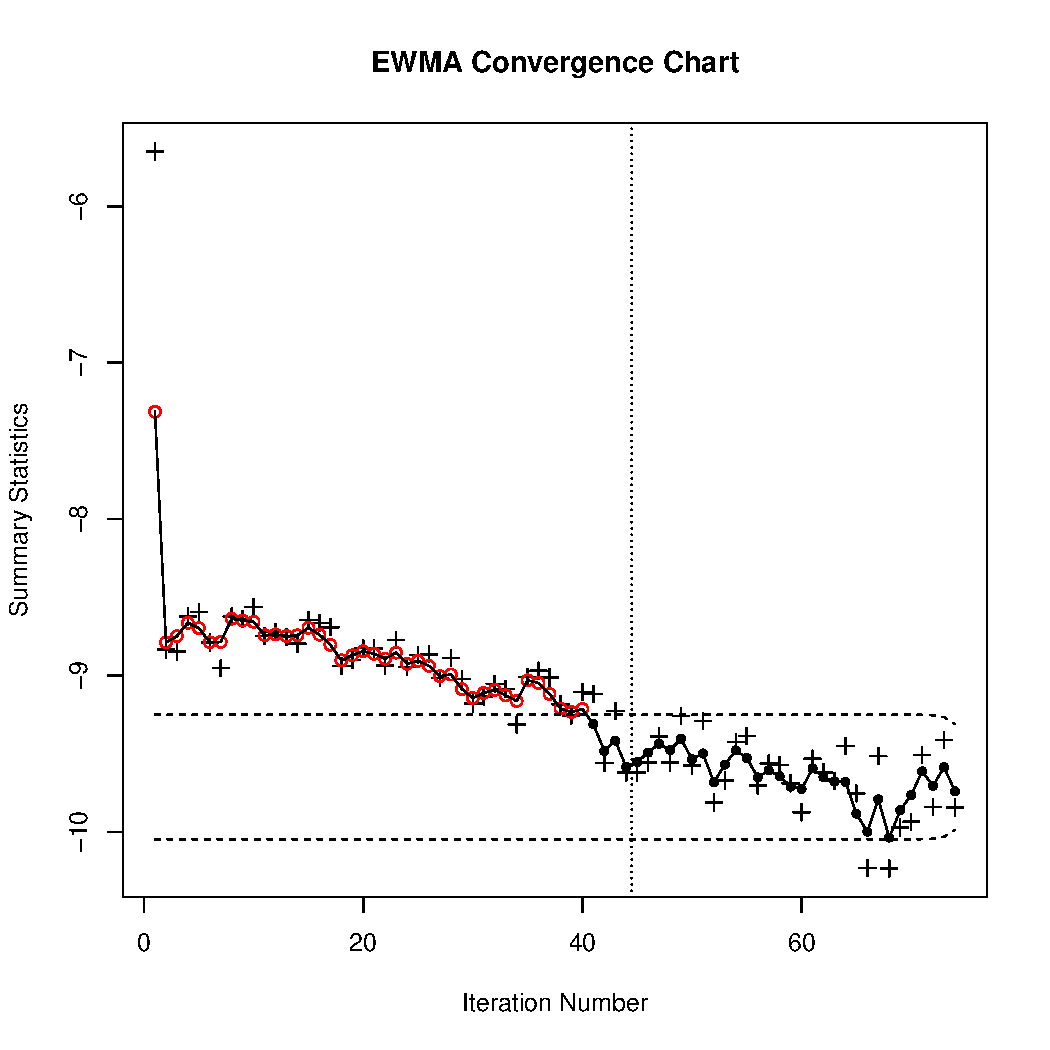
\includegraphics[width=0.32\textwidth]{./figures/ewmaConvChartRoseEasyEasyOpt.pdf}
%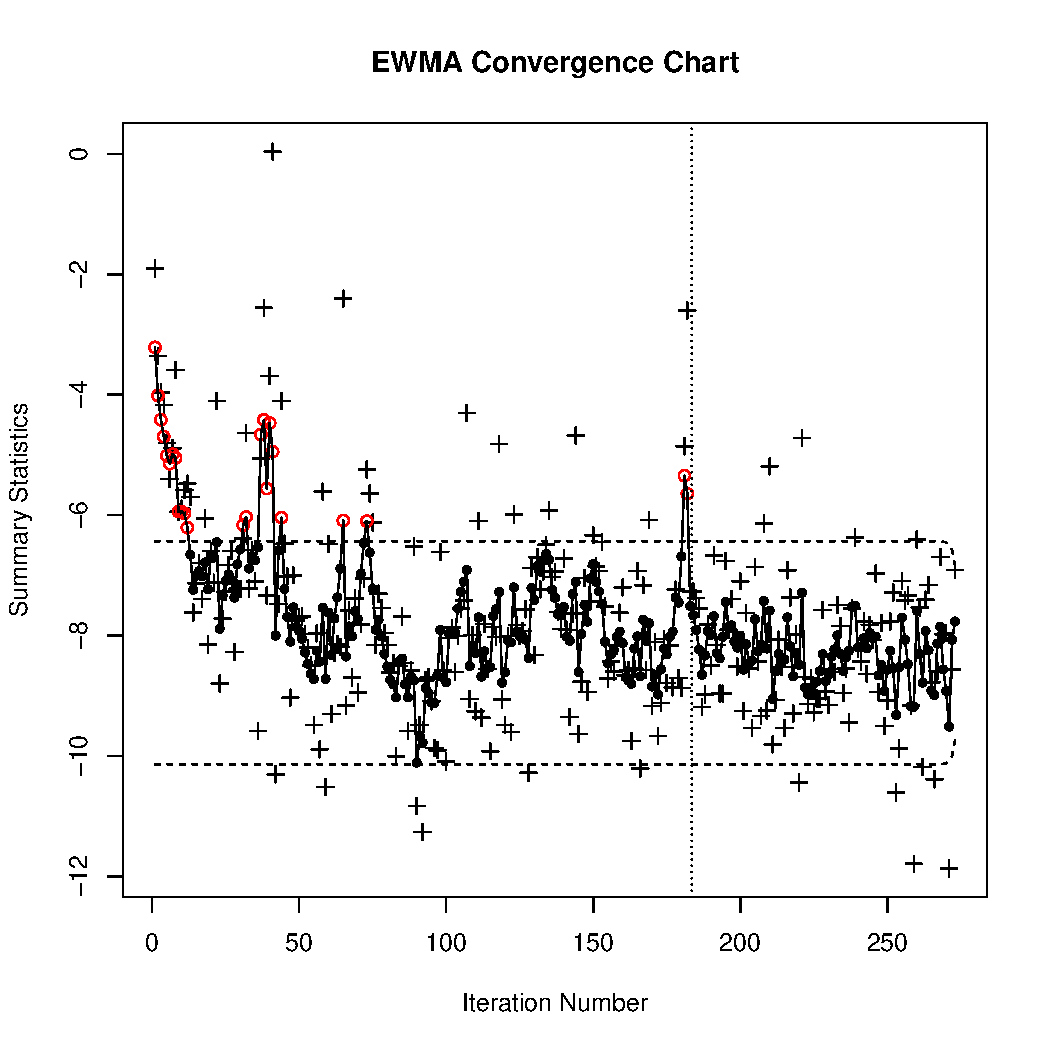
\includegraphics[width=0.32\textwidth]{./figures/ewmaConvChartLock6Three20000Opt.pdf}
%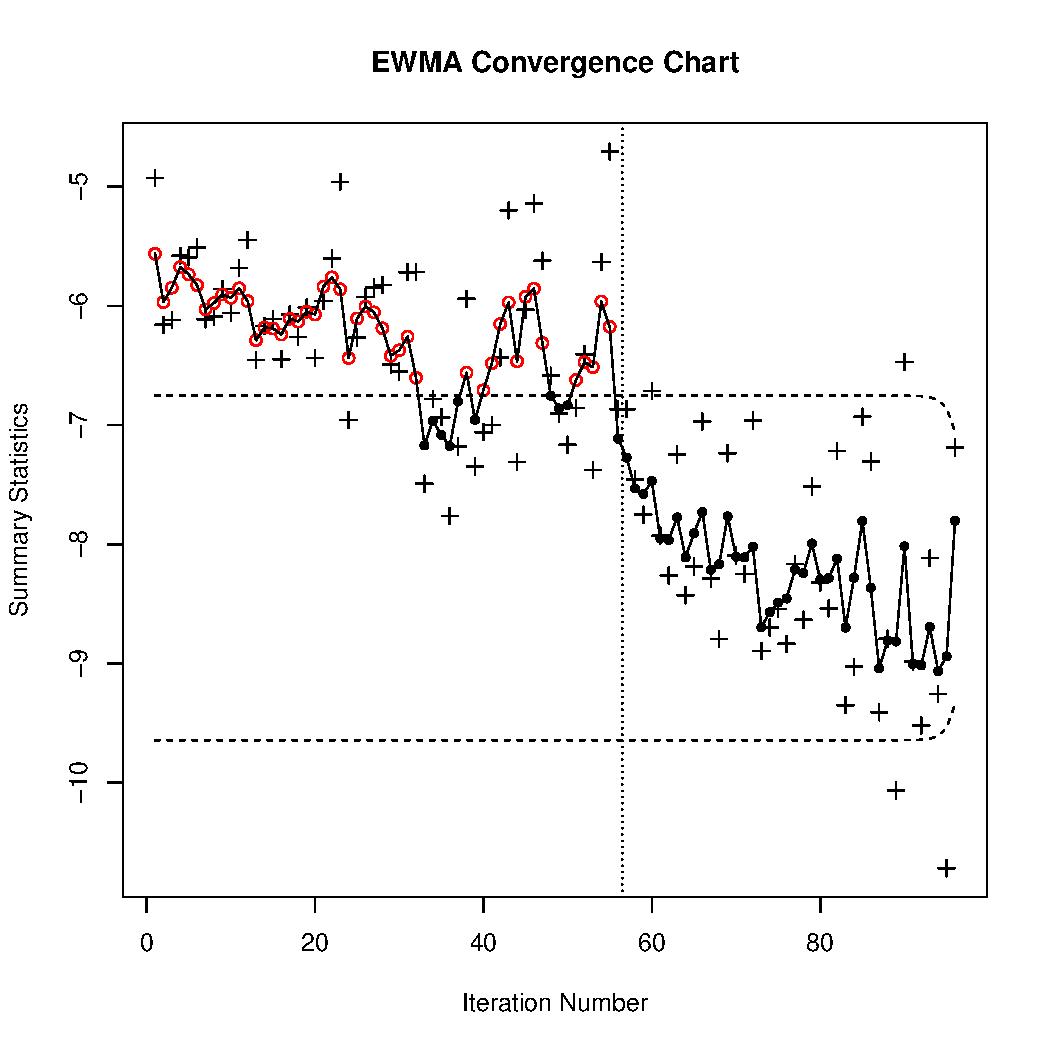
\includegraphics[width=0.32\textwidth]{./figures/ewmaConvChartRastHardOpt.pdf}
%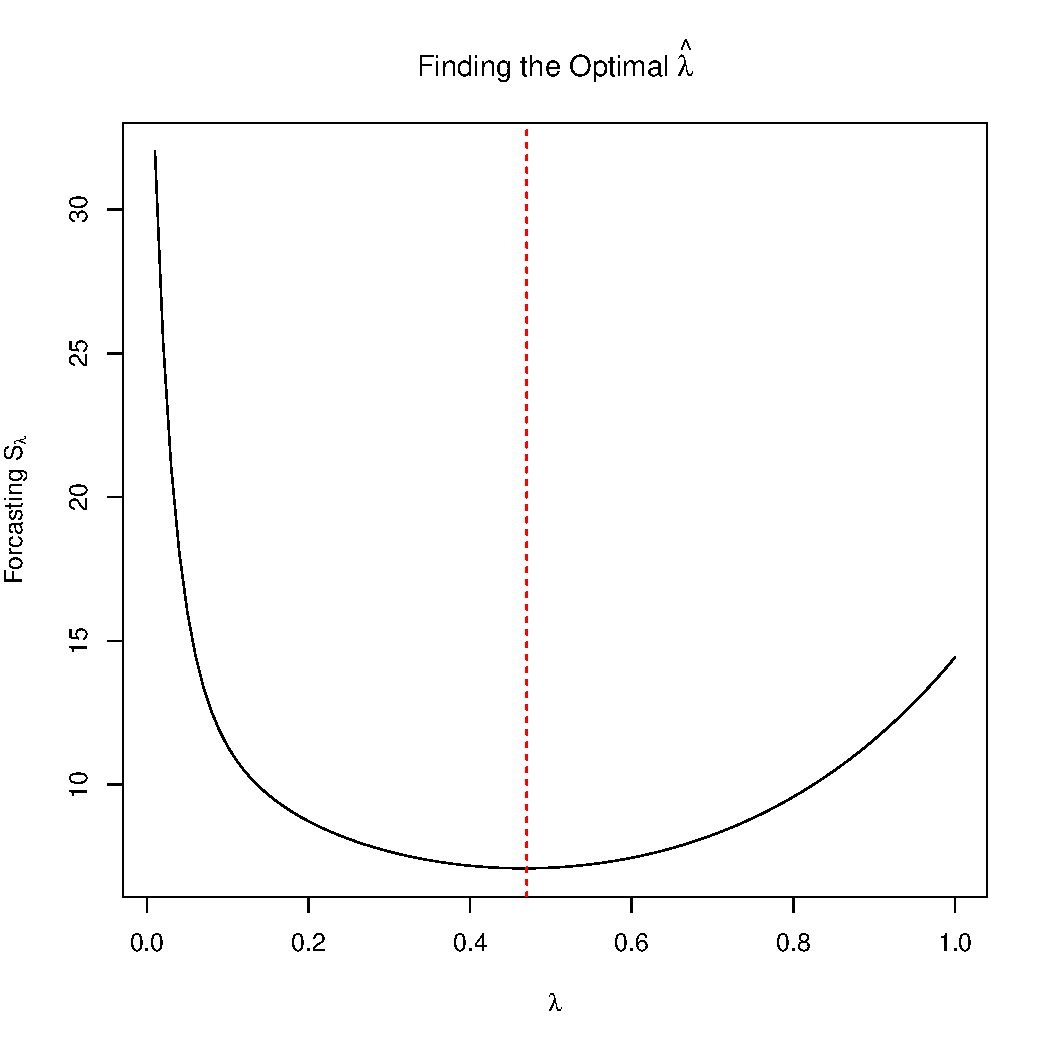
\includegraphics[width=0.33\textwidth]{./figures/ssRoseEasyEasyOpt.pdf}
%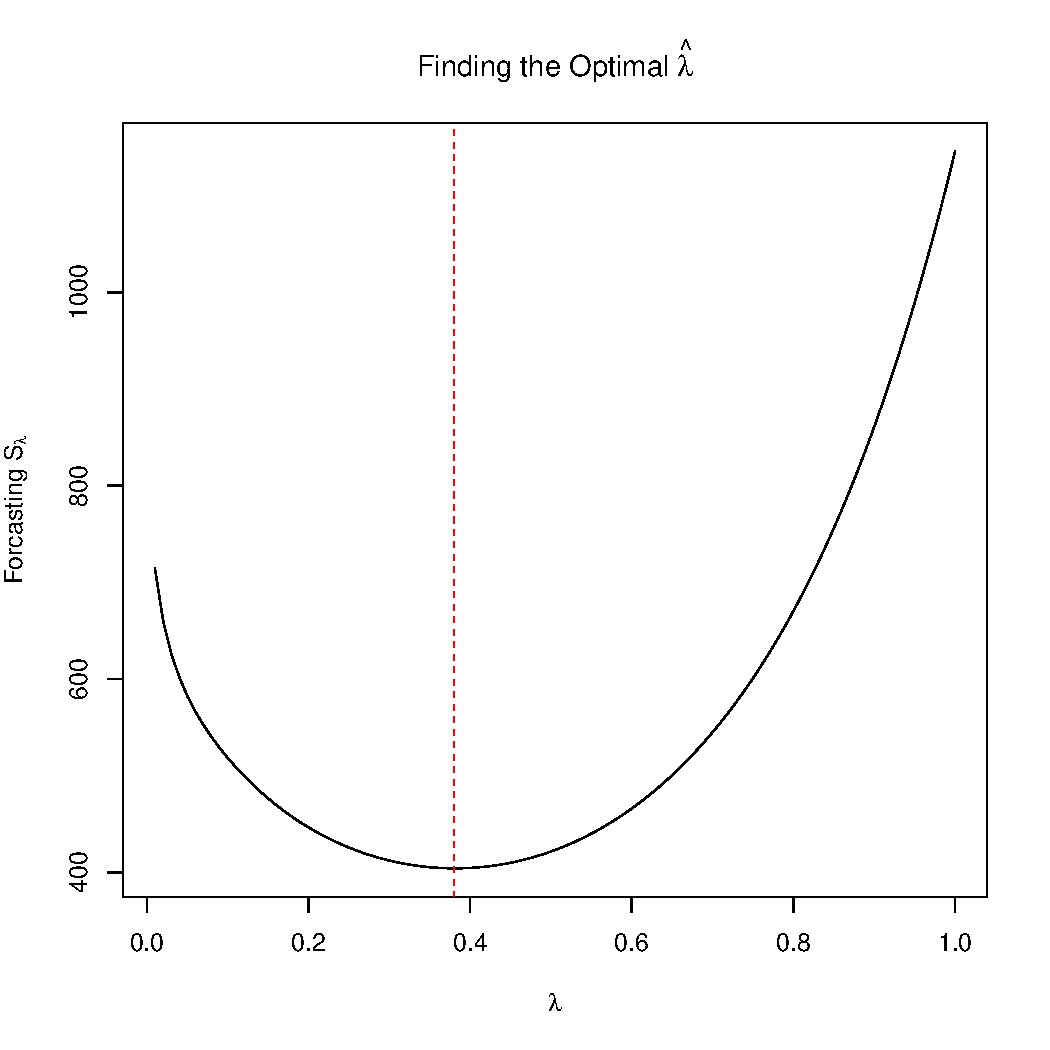
\includegraphics[width=0.33\textwidth]{./figures/ssLock6Three20000Opt.pdf}
%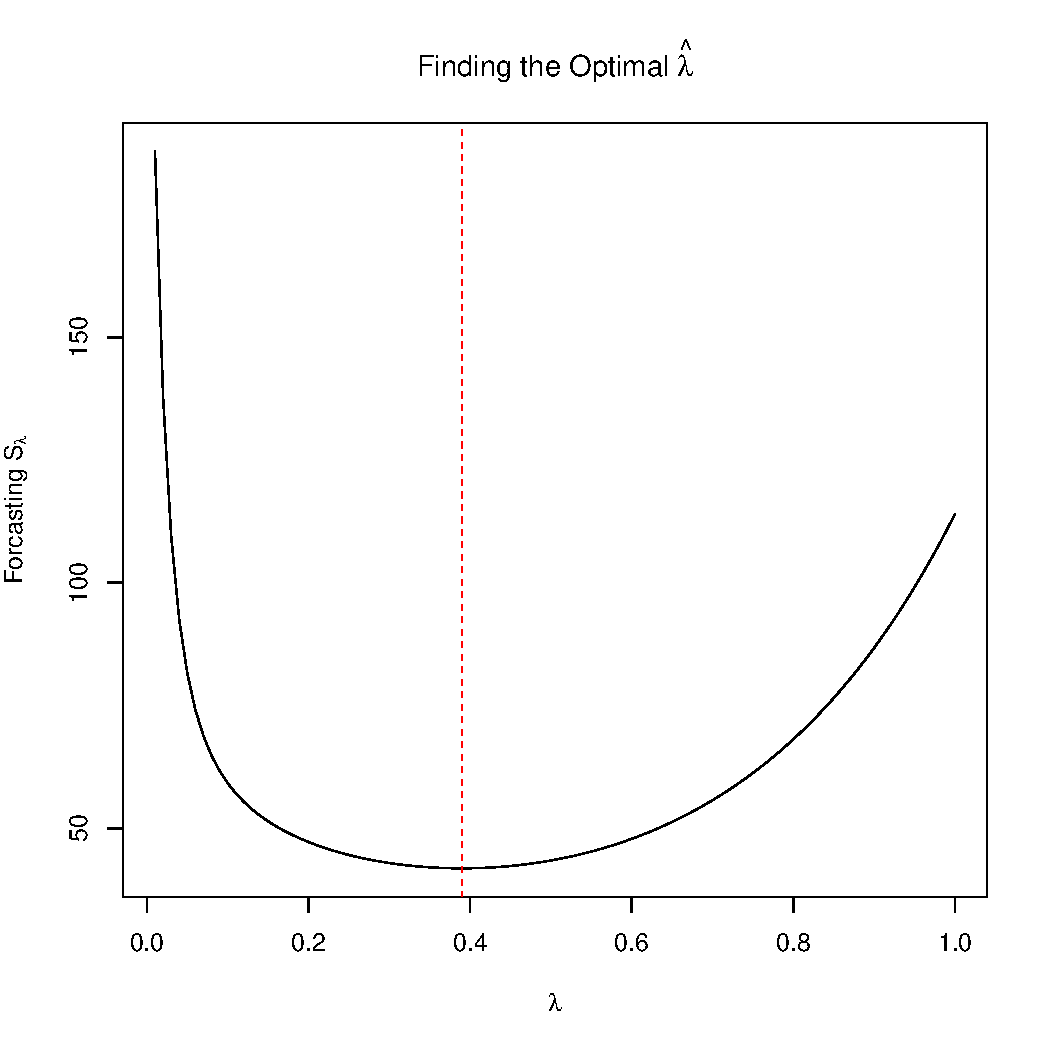
\includegraphics[width=0.33\textwidth]{./figures/ssRastHardOpt.pdf}
%\caption{$left:$ Rosenbrock | $center:$ Lockwood | $right:$ Rastrigin}
%\label{ewmaFig}
%\end{figure}
%%
%%

%
%\vspace{-0.5cm}
%\clearpage
%
%
\section{Examples}
\label{sec:examples}
%
We first look at two synthetic examples from the optimization literature, where the true optimum is known, so we can be sure we have converged to the true global minimum.  
%
We tune the EWMA Convergence Charts for each of these synthetic examples, then extrapolate the choice of $w$ to provide a real world example from hydrology.

%
%
\subsection{Rosenbrock}
%
%

%
%\begin{figure}[htb]
\begin{wrapfigure}{r}{0.41\textwidth}
%\begin{center}
        %\label{roseFig}
	\vspace{-2.25cm}
        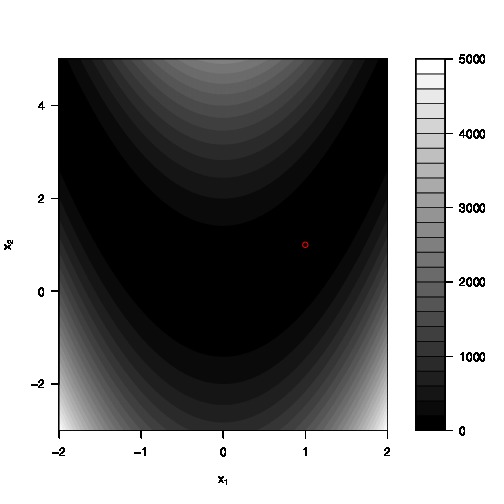
\includegraphics[width=0.5\textwidth]{./figures/roseContourBW.jpg}
	\vspace{-2cm}
        %\begin{eqnarray}
	\begin{center}
        $~~f(x_1, x_2) ~=~ 100\left(x_2-x_1^2\right)^2 + (1-x_1)^2$ \\
        $\text{Minimum}~:~~ f(1, 1)=0~~~~~~~~~~~~~~~~$%\nonumber
	\end{center}
        %\label{roseEq}
        %\end{eqnarray}  
%\end{center}
%\end{figure}
\end{wrapfigure}

%\clearpage
%
The Rosenbrock function \citep{rosePaper} was an early test problem in the optimization literature. 
%
It combines a narrow, flat parabolic valley with steep walls, and thus it can be difficult for gradient-based methods. It is generalizable to higher dimensions, but we use the two-dimensional version here.
%
Convergence is non-trivial to assess, because optimization routines can take a while to explore the relatively flat, but non-convex, valley floor for the global minimum.  
%
Here we focus on the region $-2\le x_1\le2$, $-3\le x_2\le5$.  
%
While the region around the mode presents some minor challenges, this problem is unimodal, and thus represents a relatively easier optimization problem, in the context of GP surrogate model optimization.  
%
This example illustrates a well-behaved convergence process.

%
% \clearpage
\begin{figure}[htb]
  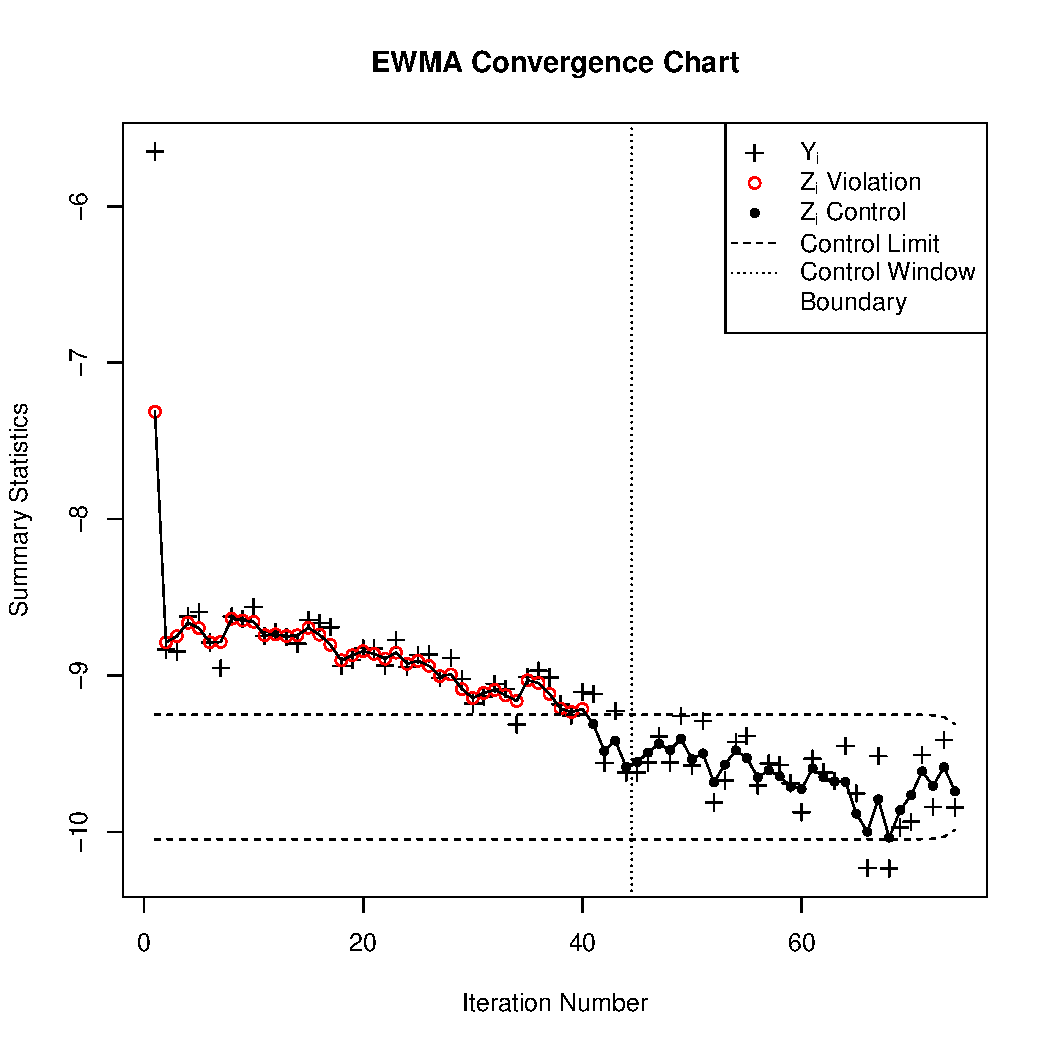
\includegraphics[width=0.45\textwidth]{./figures/ewmaConvChartRoseEasyEasyBW.pdf}
  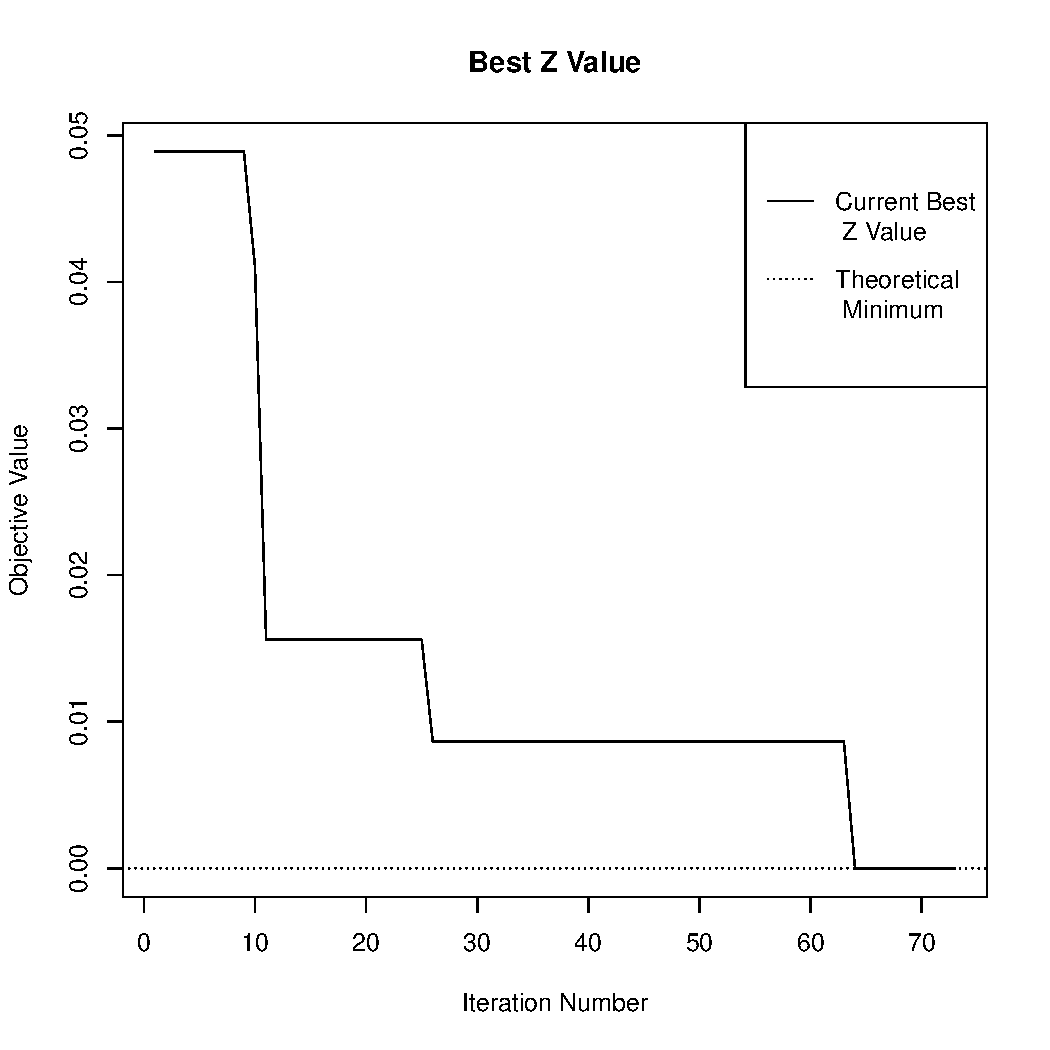
\includegraphics[width=0.45\textwidth]{./figures/bestZRoseEasyEasyEnd.pdf}
  \caption{Rosenbrock function: Convergence chart on the left, optimization progress on the right.}
\label{fig:rosenbrock}
\end{figure}
%use default values for our convergence parameters, $\lambda=0.2$ and $w=30$.
We estimate $\lambda$ via the minimum $S_\lambda$ estimator, $\hat\lambda\approx\roseLamb$.
%
Due to the relative simplicity of this problem we find that $w=30$ results in a well behaved convergence pattern with a final ELAI variance of \roseVar.
%
Figure~\ref{fig:rosenbrock} shows the result of surrogate model optimization at convergence, as assessed by our method.  
%
The right panel shows the best function value ($y$-axis) found so far at each iteration ($x$-axis), and verifies that we have found the global minimum.
%
The left panel shows the convergence chart, with the control window to the right of the vertical line, and the control limits indicated by the dashed lines.
%%
%The left panel shows our convergence chart, with the window indicated by the vertical line.  
%%
%The dashed horizontal lines show the control limits. 
%
Iteration 74 is the first time that all EWMA points in the control window are observed within the control limits, and thus we declare convergence.  
%
This declaration of convergence comes after the global minimum has been found, but not too many iterations later, just enough to establish convergence.
%
Note that the EWMA points generally trend downward until the global minimum is found at iteration 63.  

%\clearpage
%
%
\subsection{Rastrigin}
%
%

%
The Rastrigin function is a commonly used test function for evaluating the performance of global optimization schemes such as genetic algorithms \citep{rastCite}.
%
The global behavior of Rastrigin is dominated by the spherical function, $\sum_i x_i^2$, however Rastrigin has been oscillated by the cosine function and vertically shifted so that it achieves a global minimum value of 0 at the lowest point of its lowest trough at (0, 0).

%
%
\begin{center}
        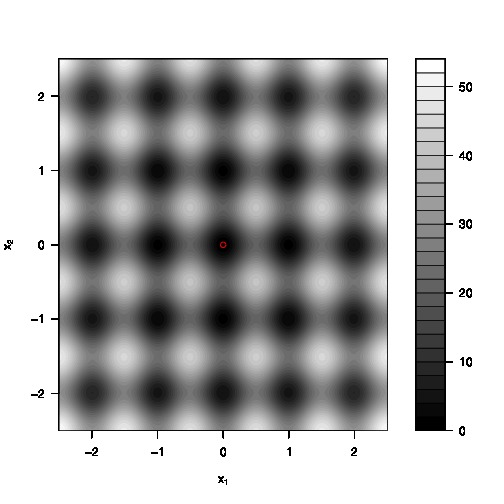
\includegraphics[width=0.5\textwidth]{./figures/rastContourBW.jpg}
        \begin{eqnarray}
        f(x_1, x_2) &=& \sum_{i=1}^2\left[x_i^2-10\cos(2\pi x_i)\right] + 2(10)\\
        \label{rastEq}
        \text{Minimum}&:& f(0, 0)=0\nonumber
        \end{eqnarray}
\end{center}
%
%

%
Rastrigin is generalizable to arbitrarily many dimensions, but to develop intuition, this example considers Rastrigin over the 2 dimensional square $-2.5\le x_i\le 2.5$.
%
Rastrigin is a highly multimodal function, and as such, the many similar modes present a challenge for identifying convergence.
%
The multimodality of this problem increases the variability of the EI criterion, and thus represents a moderately difficult optimization problem in this context. 
%
It should be noted that by increasing the size of the search domain, either by increasing the bounds of the search square and/or increasing the dimension of the domain would make this example considerably more difficult. % and a less intuitive example for developing the choice of $w$. %tuning parameters.

%
%
\begin{figure}[!htb]
        \centering
        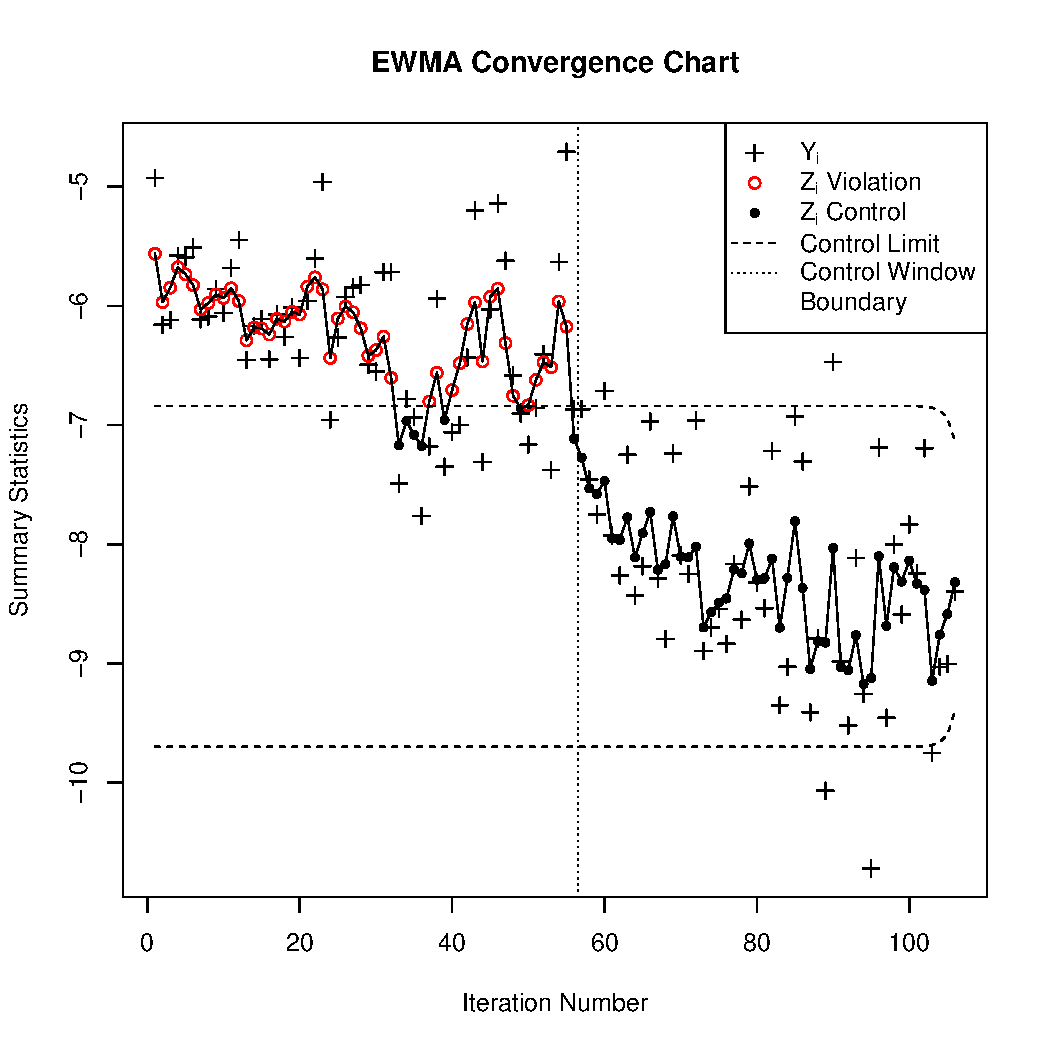
\includegraphics[width=0.45\textwidth]{./figures/ewmaConvChartRastHardEnd.pdf}
        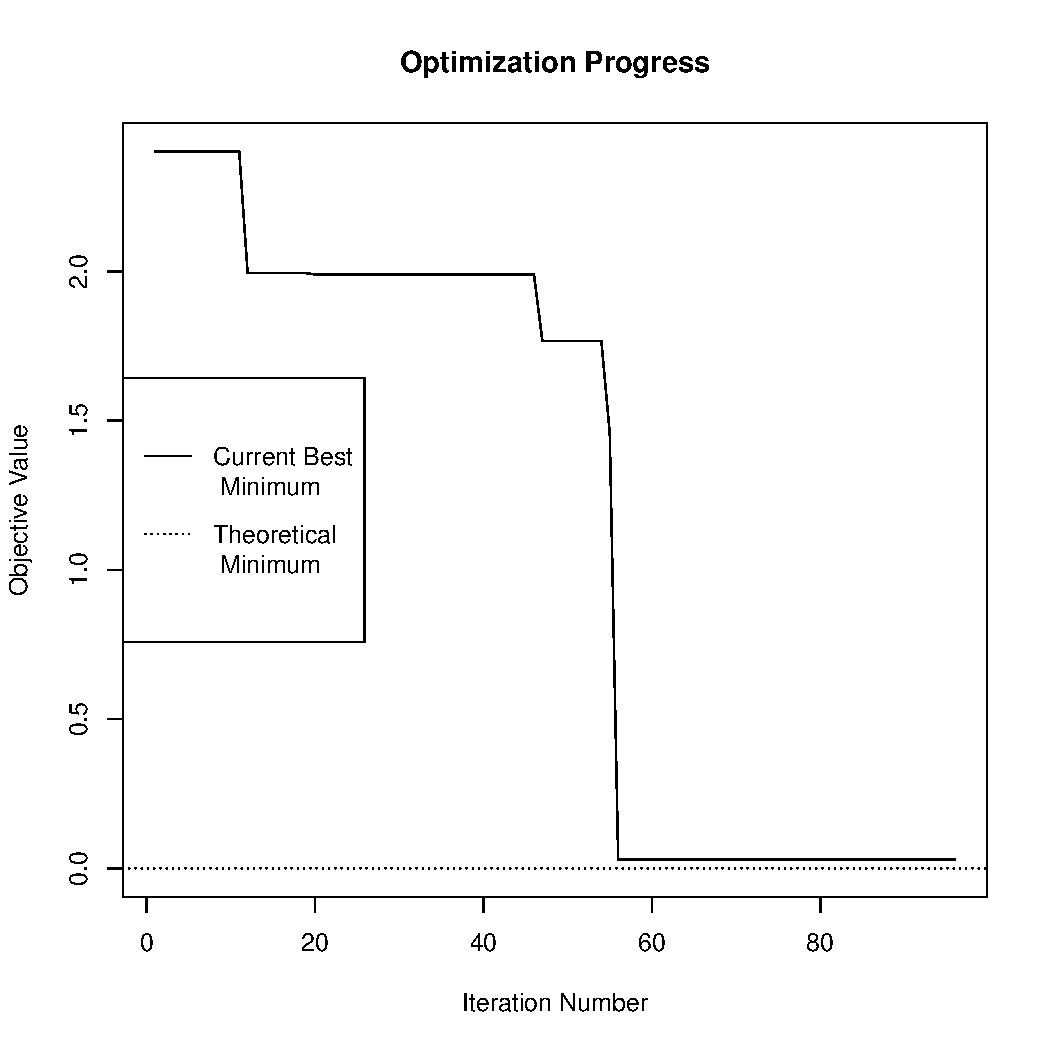
\includegraphics[width=0.45\textwidth]{./figures/bestZRastHardEnd.pdf}
        \caption{Rastrigin function: Convergence chart on the left, optimization progress on the right.}
        \label{fig:rastrigin}
\end{figure}
%
%

%
$\hat\lambda$ in this example is calculated to be about \rastLamb.
%
The decreased value of $\hat\lambda$, relative to Rosenbrock, increases the smoothing capabilities of the EWMA procedure, as a response to the increased noise in the ELAI series. %so as to separate out the increase noise in the ELAI series from  signal.% the increased noise in the ELAI series to a greater degree, as values more by reflectes the increased use of $\lambda$ as a smoothing parameter, relative to rosebrock.
%
The added noise of the ELAI series here comes from the regular discovery of dramatic new modes as optimization proceeds.
%
Due to the increased complexity of Rastrigin relative to Rosenbrock, a larger $w$ is needed to recognize convergence in the presence of increased noise in the ELAI criterion. 
%
In this application $w=50$ was found to work well, with a final ELAI variance of \rastVar.
% %
% Although larger choices of $w$ produce equally consistent identification of convergence, they do so with more function evaluations.

%
%

%
Figure~(\ref{fig:rastrigin}) shows the convergence chart (left) and the optimization progress of the algorithm (right) after 105 iterations of optimization.
%
Although the variability of the ELAI criterion increases as optimization proceeds, large ELAI values stop arriving after iteration 55, coincidently with the surrogate model's discovery of the Rastrigin's main mode, as seen in the right panel of Figure~(\ref{fig:rastrigin}).
%
Furthermore notice that optimization progress in Figure~(\ref{fig:rastrigin}, right) demonstrates that convergence in this case does indeed represent approximate identification of the theoretical minimum of the function, as indicated by the dashed horizontal line at the theoretical minimum. 

% has shown to be effective and smaller choices ofwas chosen here 
%as the  as the increased $\lambda$ attempts to forecast the large fluctuations of the ELAI criterion produced by the regular discovery of dramatic new modes.
%%
%Due to the increased complexity of the Rastrigin function a larger $w$ is needed to recognize convergence in the presence of increased noise in the ELAI criterion do to

%
%Figure~(\ref{fig:rastrigin}) 
%
%
%Notice that the  
%Due to the increased complexity of the Rastrigin function a larger $w$ is needed to recognize convergence in the presence of increased noise in the ELAI criterion do to 

%%
%\begin{itemize}
%%\item lambda choice
%%\item w choice
%\item results (when,where,bestZ fig)
%\item interesting tid-bits
%\end{itemize}

%
%
\subsection{Lockwood Case Study}
\label{sec:lockwood}
%
%

%closed form
The previous examples have focused on analytical functions with known minima.
%
This is done for the sake of developing an intuition for tuning the EWMA convergence chart parameters and to ensure that our methods correspond to the identification of real optima.
%However, in most practical optimization problems it is not possible to visualize to objective function so straight forwardly, or derive theoretical minima in this way.
%REVISE!!!!
%To demonstrate the use of the EWMA convergence chart in a practical optimization problem, 
Here we apply the EWMA convergence chart in the practical optimization setting of pump and treat optimization problems as formulated by \cite{mayer2002optimal}.
%
Specifically we consider the Lockwood pump and treat problem, originally presented by \cite{lockCite}. %, and additionally presented \cite{gramacy2014}.

%
%

%%of contaiminted groundwater tha pumping site for chlorinated solvents located north-east of Billings, Montana, along the Yellowstone River.

The Lockwood pump and treat case study considers an industrial site, along the Yellowstone River in Montana, with groundwater contaminated by chlorinated solvents. %cothat has contaminated the surrounding groundwater with chlorinated solvents.%
%
If left untreated, this contaminated groundwater may contaminate the Yellowstone river, as dictated by the hydrology of the system. %ical models.
%Yellowstone river the site is close enough to the contaminate the Yellowstone river with  Chlorinated solvents contaminating the ground water in this region  , two plumes for pumping
In order to control this contaminated groundwater, a total of six pumps, situated over two plumes of the contaminated groundwater are used to redirect groundwater away from the river to a treatment facility.
%
Due to the cost of running these pumps, it is desirable to determine how to best allocate the pumping effort among these pumps so as to determine the lowest cost pumping strategy to protect the river.
%
Pumping each of these six wells at different rates can drastically change the groundwater behavior, and  thus a numerical simulation of the system is required to predict the behavior of the system at a given set of pumping rates. %behavior of the of the ground%results in changes the complicated groundwater behaviors, that require the evaluation of a numerical simulation of the system to predict.
%
% from the groundwater does not reach the Yellowstone River.
%Plumes A and B contain two and four wells respectively.
%seen in Figure (\ref{lockSite}), contains two plumes for pumping, Plume A and Plume B, containing two and four wells respectively.
%
%The objective is to determine the lowest cost pumping rates for each of these six wells such that contamination from the plumes does not reach the Yellowstone River.

%
%

%
The objective function, $f(\bm{x})$, to be minimized in this case, can be expressed as the sum of the pumping rates for each pump (a quantity proportional to the expense of running the pumps in USD), with additional large penalties associated with any contamination of the river. % by each plume, $c_A(\bm{x})$, $c_B(\bm{x})$. %$c_A(\bm{x})$ and $c_B(\bm{x})$ indicating that the  
        %, is the cost of operating the pumps, in USD; additionally, $f$ heavily penalizes solutions that contaminate the river.
\begin{equation}
f(\bm{x}) = \sum_{i=1}^6 x_i +  2\big[ c_a(\bm{x}) + c_b(\bm{x}) \big] + 20000 \big[ \oner_{c_a(\bm{x})>0} + \oner_{c_b(\bm{x})>0} \big] 
\label{lockLoss}
\end{equation}
%with simple search boundaries, \mbox{$0\le x_i\le20,000$} set for each pumping rate.
Here $c_a(\bm{x})$ and $c_b(\bm{x})$ are outputs of a simulation, indicating the amount of contamination, if any, of the river as a function of the pumping rates, $\bm{x}$, for each of the six wells.
%
Any amount of contamination of the river results in a large stepwise penalty which introduces a discontinuity into the objective function, at the contamination boundary.
%Penalties associated with any contamination of the river are chosen to be large, so as to never gi enough to 
%
%, \mbox{$\left[x_1, ..., ~x_6\right] = \left[Q_{A1}, ~Q_{A2}, ~Q_{B1}, ~Q_{B2}, ~Q_{B3}, ~Q_{B4}\right]$}.
Each $x_i$ is bounded on the interval \mbox{$0\le x_i\le20,000$}, representing a large range of possible management schemes.
%
The full problem defines a six-dimensional optimization problem to determine the optimal rate at which to pump each well, so as to minimize the loss function defined in Eq~(\ref{lockLoss}).
%
Since the loss function is defined over a large and continuous domain, and running the numerical simulation of the system is computationally expensive, this example presents an ideal situation for use with surrogate model based optimization. 
%to understand the behavior of the EI criterion I first consider simplified into%with respect to $f$;
%The two-dimensional problem provides a nice setting for understanding the a simplified version of EI behavior, and furthermore the simplified setting develops an expectation for the EI behavior in the full \mbox{six-dimensional problem.}



% \begin{itemize}
% \item Describe case study
% \item general shape characteristics os loss function
% \end{itemize}
% 
% %
% {\color{red} insert loss function, and some visualization}
% \begin{equation}
% f(\bm{x}) = \sum_{i=1}^6 x_i +  2\big[ c_A(\bm{x}) + c_B(\bm{x}) \big] + 20000 \big[ \oner_{c_A(\bm{x})>0} + \oner_{c_B(\bm{x})>0} \big] 
% \end{equation}
%

%\begin{itemize}
%%\item describe search domain
%\item ~~~ describe challenges ~~~
%\end{itemize}

%
%%ewmaConvChartLock6Three20000.pdf
\begin{figure}[htb]
        \centering
        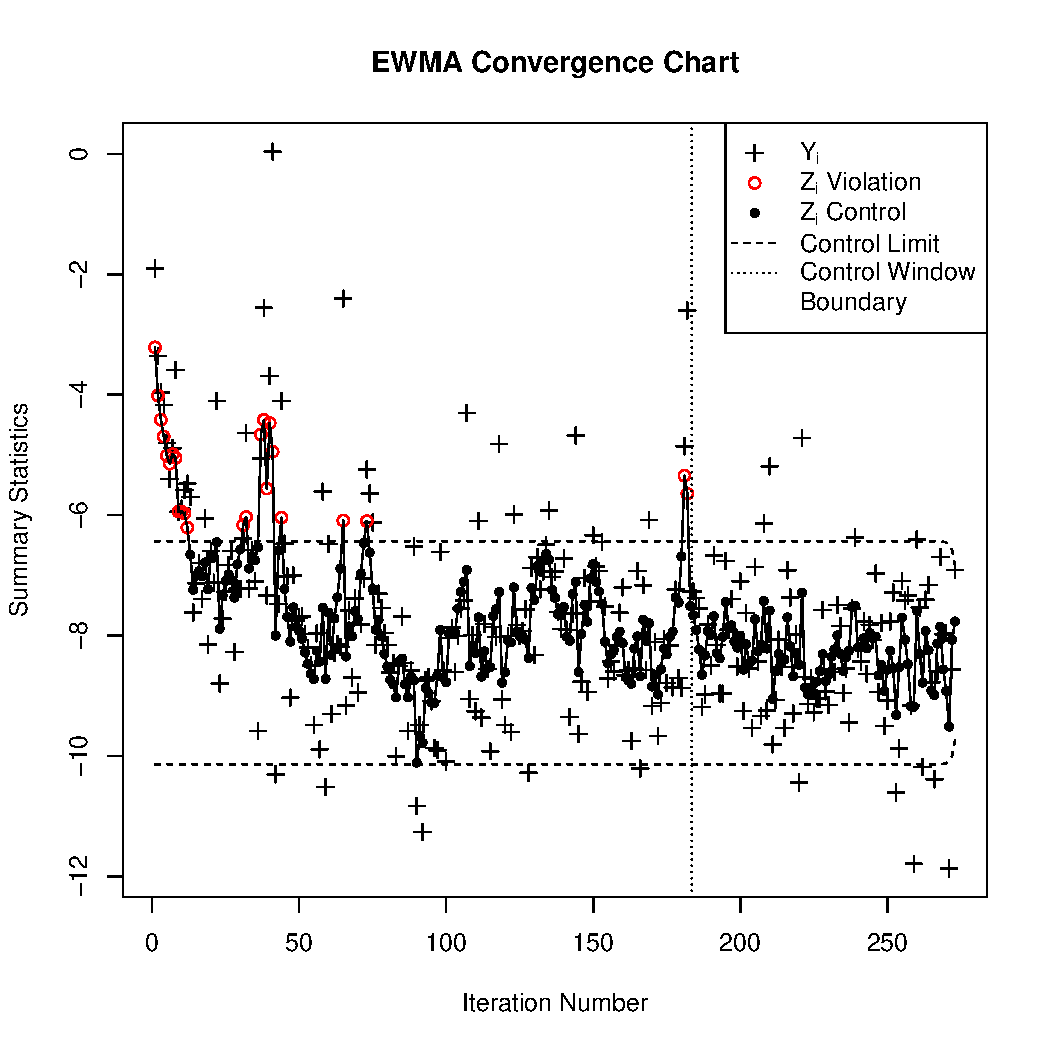
\includegraphics[width=0.45\textwidth]{./figures/ewmaConvChartLock6Three20000End.pdf}
        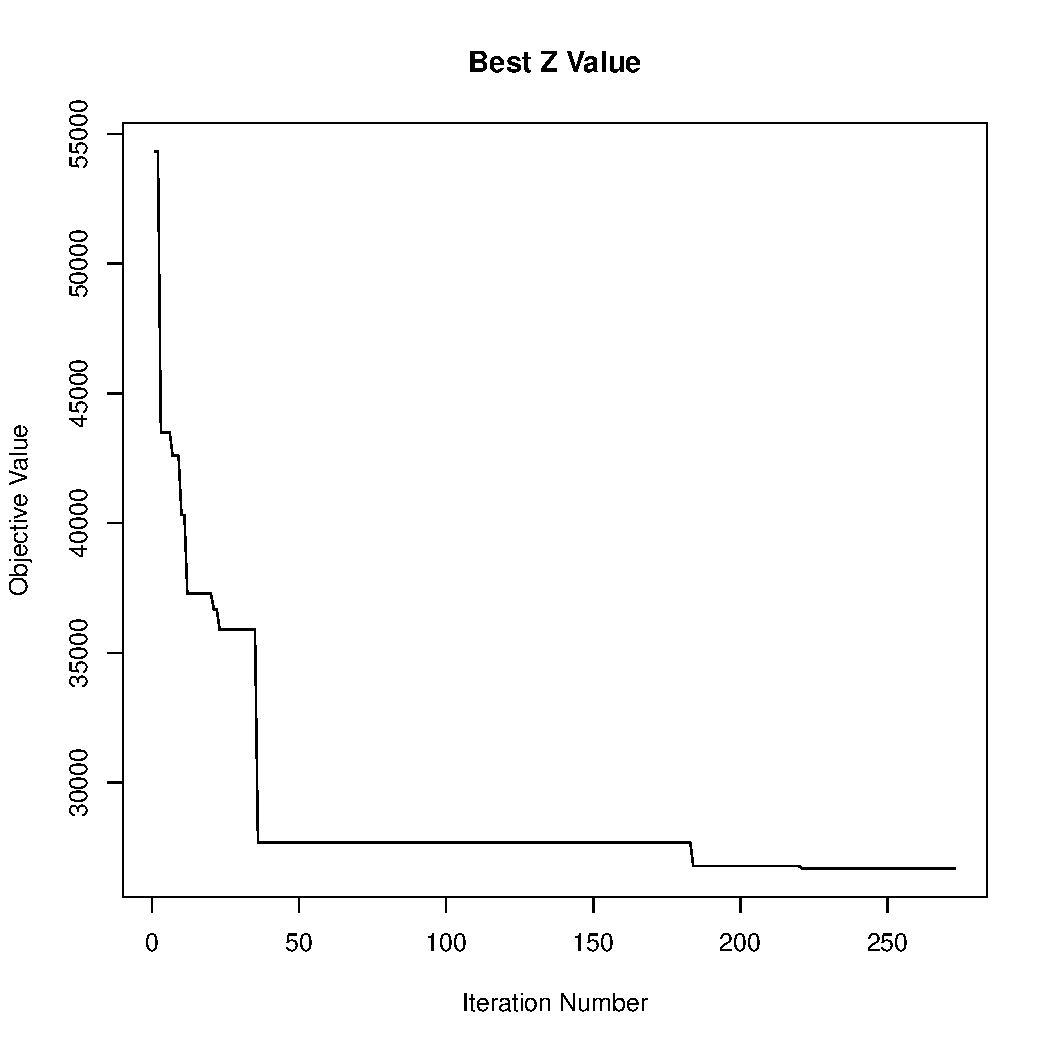
\includegraphics[width=0.45\textwidth]{./figures/bestZLock6Three20000End.pdf}
        \caption{Lockwood Case-study: Convergence chart on the left, optimization progress on the right.}
        \label{lock6EWMAEnd}
\end{figure}
%
%

%
By using the fitted values of $w$ and the observed ELAI variance in each of the two previous examples we extrapolate an apporpriate value of $w$ for this case study based on an observed ELAI variance of \lockVar, resulting in an estimated $w$ of $93\approx\left(\frac{50-30}{\rastVar-\roseVar}\right)\lockVar+30$, as discussed in section 3.4.
%
Again $\lambda$ was chosen via the minimum $S_\lambda$ estimator to be $\hat\lambda\approx\lockLamb$ in this case. 
%
This level of smoothing is required here to reduce the noise in the ELAI criterion due to the large search domain, as well as the complicated contamination boundary among the six wells.
%
Furthermore these features of the objective function complicate fit of the surrogate model and thus more function evaluations are required to produce an accurate model of $f$.


% %
% By using the fitted values of $w$ and the observed ELAI variance in each of the two previous examples we extrapolate an apporpriate value of $w$ for this case study based on the observed ELAI variance of $\hat v_{lock}\approx\lockVar$ in sample runs of the lockwood simulation. 
% The estimated log linear relationship between $w$ and the ELAI variance produces $\hat \beta_1\approx0.62$ and $\hat \beta_0\approx3.36$ resuting in an estimated $\hat w_{lock}\approx e^{\hat\beta_0}\exp\{\hat\beta_1~v_{lock}\}=99$. 
%$99\approx\exp\bigg\{\left(\frac{\log(50)-\log(30)}{0.88-0.06}\right)(\lockVar-0.06)+\log(30)\bigg\}$ 
%an observed ELAI variance of \lockVar, resulting in an estimated $w$ of $99\approx\left(\frac{60-30}{\rastVar-\roseVar}\right)\lockVar+30$, as discussed in section 3.4.

%\clearpage
 %  accurately  the of the  dificultie
% to get a enough information to provide  to gather enough information to  was chosen to be 90 iterations of the algorithm to provide the 
%to produce, to yield
% As a result, the control window size, $w$, must increase to provide the initial surrogate model enough information to yield reasonable accuracy. 
% %determined, demonstrated, established, indicated, validated, corroborated
% Here $w$ was chosen to be 90 iterations, as determined by the adequate initial surrogate model behavior. % as well as consistent identification of convergence.

%
%

%
The convergence chart for monitoring the optimization of the Lockwood case study is shown in the left panel of Figure~(\ref{lock6EWMAEnd}), as computed with $\hat\lambda\approx\lockLamb$ and $w=93$. %  $ (left) and optimization progress
%
Convergence in this case does not occur with a dramatic shift in the mean level of the ELAI criterion, but rather convergence occurs as the series stabilizes after large ELAI values move beyond the control limit. %, and  
%
Interestingly the last major spike in the ELAI series is observed alongside the discovery of the final major jump in the current best minimum value as seen at about iteration $180$ in the right panel of Figure~(\ref{lock6EWMAEnd}).
%
The EWMA convergence chart identifies convergence as the EWMA statistic associated with this final ELAI spike eventually exits the control window at iteration $276$.
%
The solution shown here corresponds to $f(\bm{x})\approx26696$ at $\bm{x}\approx[0, 6195, 12988, 3160, 1190, 3163]$.
%
This solution is well corroborated as a point of diminishing returns for this problem, by the analysis of \cite{gramacy2014} on the same problem, as seen in their average EI surrogate modeling behavior. %gorithms as guided by the EI criterion.
%In Figure (18, right), after about 210 iterations, the algorithm finds its lowest cost solution to be seen in 500 iterations, corresponding to f (x) ≈ 26696 at x ≈ [0, 6195, 12988, 3160, 1190, 3163]. 
%Considering Figure (18, left), the EWMA convergence chart identifies this convergence after only about 270 iterations.
%%
%%
%%
%Figure~(\ref{fig:rastrigin}) shows the convergence chart (left) and the optimization progress of the algorithm (right) after 95 iterations of optimization.
%%
%Although the variability of the ELAI criterion increases as optimization proceeds, large ELAI values stop arriving after iteration 55, coincidently with the surrogate model's discovery of the Rastrigin's main mode, as see in the right panel of Figure~(\ref{fig:rastrigin}).
%%
%Furthermore notice that optimization progress in Figure~(\ref{fig:rastrigin}, right) demonstrates that convergence in this case does indeed represent approximate identification of the theoretical minimum of the the function, as indicated by the dashed horizontal line at the theoretical minimum. 

%
%\begin{itemize}
%%\item lambda choice
%%\item w choice
%\item results (when,where,bestZ fig)
%\item interesting tid-bits
%\end{itemize}
%

%
%
\section{Conclusion}
%
%

%
Adapting the notion of control from the SPC literature, the EWMA convergence chart outlined here aims to provide an objective standard for identifying convergence in the presence of the inherent stochasticity of the improvement criterion in this setting. %provides an objective definition of convergence. 
%
The examples provided here demonstrate how the EWMA convergence chart may accurately and efficiently identify convergence in the context of GP surrogate model optimization. 
%
We note that our approach could be applied with any optimization algorithm that allows computation of an expected improvement at each iteration.

%
%

%characterization; consideration
As for any optimization algorithm, a converged solution may only be considered as good as the algorithm's exploration of $f$. 
%
Thus poorly tuned surrogate modeling strategies may never optimize $f$ to their fullest extent, but the EWMA convergence chart presented here may still claim convergence in these cases. % algorithms. 
%
The EWMA convergence chart may only consider convergence in the context of the algorithm in which it is embedded, and thus should be interpreted as a means of identifying when an algorithm has converged rather than when the lowest minimum has been found. % only identify convergence relative to the quality
%
%In cases of poorly tuned algorithms, the EWMA convergence chart presented here may only identify convergence with respect to the quality of the particular surrogate modeling strategy used. 
%may often 
For poorly tuned surrogate modeling strategies the EWMA convergence chart may only identify that the algorithm has reached a point of diminishing returns, or that it has converged to a local mode; for well-tuned surrogate modeling strategies, this point should correspond with the realization of an optimal solution. 
%
In either case, the EWMA convergence chart identifies the moment at which it is beneficial to stop iterating the routine and reflect upon the results.

%
%

%%
%Of course the methods shown here are not presented in the absence of their own parameters that require tuning, But I view these added parameters in Archemedies' spirit of replacing hard problems with a series of easier ones. 
%%

%
%{\color{red} SOME METHODOLOGY IMPROVEMENT SENTENCE }
The EWMA convergence chart presented here is intended as a starting point for establishing an appropriate analysis of convergence for sequential surrogate modeling optimization algorithms.
%for these algorithms will remain fundamental to any appropriate characterization of convergence here.
Details of the particular implementation of these methods may improve through further analysis of model usage and parameter estimation. 
%
% transformed improvement distributions with
The strategy presented here for transforming the improvement distribution via the Log-normal approximation to the improvement distribution has shown to be an empirically effective and computationally simple solution to better meet the assumptions of the EWMA control charting methodology.
%
However, some applications may find it worthwhile to explore other transformations which could result in higher overall transformed signal to noise ratios, across a more broad set of improvement distributions. %s which may result in a in a more effective use of the information in the improvement distribution.
%
For example, rather than adopting the ELAI transformed estimate from the improvement distribution, it may be computationally feasible to apply the two-parameter Box-Cox transformation \citep{boxCox1964} to the improvement samples,
\begin{equation}
y_i^{(\bm{\lambda})}~=~
\begin{cases}
        \frac{( y_i + \lambda_2 )^{\lambda_1} - 1}{\lambda_1} & \lambda_1\neq0\\
        \log(y_i+\lambda_2) & \lambda_2=0
\end{cases}
\end{equation}
thus alleviating any difficulties due to numerical truncation of the improvement samples at 0, while finding a flexible transformation to reduce skew.
%
It should be noted that this approach adds additional computational expense, while our ELAI transformation requires minimal computation.   
%furthermore
Additionally the EWMA convergence chart could benefit from a more precise method for choosing the control window size parameter, $w$, although developing such a method would be a major research project itself; our empirical solution has worked well in practice.
%
Although improvements to the details of these methods may exist, the fundamental consideration of the stochastic nature of convergence in this setting would remain, and SPC offers a nice framework for its inclusion. %, through SPC or otherwise, should remain for an appropriate characterization of convergence here.

%
%

%
%This analysis makes
%
%The EWMA conv
%%
%The strategy shown here for transforming  tuning λ and w demonstrates an empirically effective ap-
%proach for tuning the EWMA convergence chart parameters. 
%%
%This approach is mainly useful due to its simplicity, although other more pointed methods may surely calculate more effective values.
%λ


%%
%Admmitadly the use of the EWMA convergence chart comes with the addition of it's own parameters which themselves require estimation.
%% 
%The addition of these parameters can be easily justified under a divide and conquer mentality; thus replacing the original large subjective task of appropriately identifying convergence with relatively simple parameter estimation problems. 
%%
%The choice of $\lambda$ has been shown to be relatively robust to suboptimal choices, and furthermore estimation of the minimum sum of the squared forecasting errors $\hat\lambda$ is a simple in practice.
%%
%The estimation of $w$ is more subtle, but follows from reasonable intuition of the problem.
%%
%The choice of $w$ would ideally consider an objective measure of the complexity of $f$ as well as the dimensionality of the domain, $p$.
%%
%%Fully characterizing the relationship between $w$ and the dimensionality and complexity of $f$ for choosing would require a large simulation experiment many possible objective function   
%%
%For simplicity the recommendation $w\ge15p$ has shown to work quite well, although it contains no explicate consideration of the observed complexity of $f$. 
%%The rational being that the current methods for appropriate identification of convergence is a rather subjective task and 
%%The choice of the EWMA convergence chart parameters, $w$ and $\lambda$,  
%%Tuning the parameters 
%%These methods are not presented in the absence of 

%\begin{itemize}
%\item tuning parameters added in the spirit of reducing hard problems into a series of easier ones
%       \begin{itemize}
%       \item convergence is hard and massively subjective
%       \item interpreting convergence charts is easier
%       \item tuning $\lambda$ is objective and robust
%       \item tuning $w$ can be subjective (requires large simulation study to choose.)
%       \end{itemize}  
%\item choose $w$
%       \begin{itemize}
%       \item complexity of $f$ (??entropy??)
%       \item Dimension of $f$
%       \item Emplerical results here: $w\approx 15p$; $p$ is the dimension
%       \end{itemize}
%{\color{red}
%\item 2-parameter box-cox EI transformation instead of ELAI}
%\end{itemize}

\clearpage
%
%
\section{Appendix}
%
%

\section*{ewmaFunc.r}
\spacingset{0.8}
\VerbatimInput{ewmaConvChart.r}
\clearpage
\spacingset{1.45}
\section*{main.r}
\spacingset{0.7}
\VerbatimInput{example.r}
\spacingset{1.45}

%
%
\clearpage
%\newgeometry{ margin=1in, top=0.6in, footskip=0.4in }
\singlespacing
\bibliographystyle{jasa}
\bibliography{./spcCite}
%
%

\end{document}



